\documentclass[titlepage]{article}
\usepackage{algorithm}
\usepackage{algpseudocode}
\usepackage{amsfonts}
\usepackage{amsmath}
\usepackage{geometry}
\usepackage{hyperref}
\usepackage{pgfplots}
\usepackage{xparse}
\usetikzlibrary{shapes,matrix}
\geometry{margin=1.2in}
\hypersetup{
  colorlinks,
  citecolor=black,
  filecolor=black,
  linkcolor=black,
  urlcolor=black
}
\pgfplotsset{compat=1.9}
\setcounter{secnumdepth}{5}
\setcounter{tocdepth}{5}
\title{%
  Artificial Neural Networks (work in progress draft) \\
  \large Getting Up To Speed With The Math From Scratch
}
\author{Attila M. Magyar}
\begin{document}
\begin{titlepage}\maketitle\end{titlepage}

  \tableofcontents

\newpage

  \section{Introduction}

    I decided to brush up my knowledge on the math behind artificial neural
    networks, and these are the notes that I've taken along the way.

    The appendix contains a collection of notations, definitions, and theorems
    from the fields of linear algebra and calculus that are used throughout
    this document.

\newpage

  \section{Neurons and Neural Networks}

    \subsection{Neuron}

      An artificial neuron is a mathematical model that captures the behaviour
      of a real, biological brain cell called a "neuron".

      \begin{figure}[!htb]
        \centering
        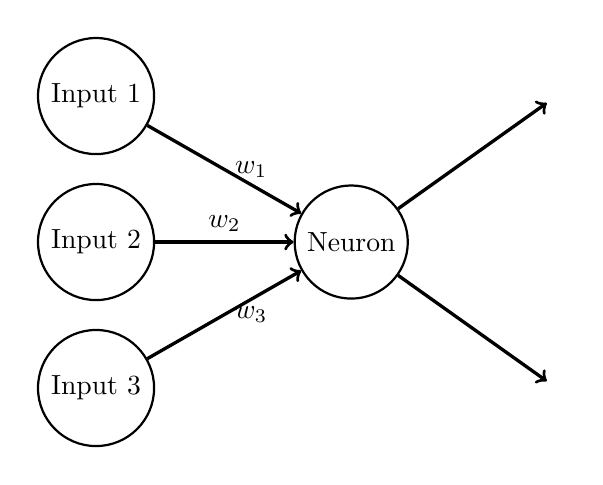
\begin{tikzpicture}[
          neuron/.style={
            circle,
            thick,
            draw=black,
          },
        ]
          \matrix[row sep=1em, column sep=5em]{%
            \node[neuron](i1){Input 1}; & & \node(o1){ }; \\
            \node[neuron](i2){Input 2}; & \node[neuron](n){Neuron}; & \\
            \node[neuron](i3){Input 3}; & & \node(o2){ }; \\
          };
          \draw
              (i1) edge [->,very thick] node[above,right]{$w_1$} (n)
              (i2) edge [->,very thick] node[above]{$w_2$} (n)
              (i3) edge [->,very thick] node[below,right]{$w_3$} (n)
              (n) edge [->,very thick] (o1)
              (n) edge [->,very thick] (o2);
        \end{tikzpicture}
        \caption{%
          A neuron with 3 input connections with various weights,
          and 2 output connections.
        }
      \end{figure}

      A real neuron may have incoming connections from other neurons and
      sensing organs, and outgoing connections to other neurons, muscles, etc.
      Depending on its inner state and the signals that it receives from its
      inputs, a neuron may or may not send a signal to its outputs, and if it
      does send a signal, the strength of that can also vary. The strength of
      the outgoing signal is called the "activation" level of the neuron.

      A mathematical neuron's activation is represented by a number,
      $a \in \mathbb{R}$.

      For a neuron with no incoming connections (called an "input" neuron, also
      known as "feature"), the activation is determined by the raw input data,
      for example, a single pixel's luminosity level in photo, scaled to the
      $[0, 1] \subset \mathbb{R}$ interval.

      For neurons with $n \in \mathbb{N}^+$ incoming connections, the
      activation is calculated as a function of the sum of the neuron's own
      bias parameter $b \in \mathbb{R}$ and the weighted sum of the activations
      of all the neurons from which an incoming connection to this neuron
      exists, with some function $f : \mathbb{R} \rightarrow \mathbb{R}$ called
      the "activation function" ($\mathbf{a}, \mathbf{w} \in \mathbb{R}^n$):

      \begin{equation}
        a = f \left( b + \sum_{k=0}^n w_k \cdot a_k \right)
      \end{equation}

      The weights and biases for a collection of neurons are usually calculated
      by a training algorithm, which, based on the derivative of the activation
      function, will arrange the parameter values so that for a given set of
      input activations, the neurons will produce the desired output
      activations.

      \subsubsection{Common activation functions and their derivatives}

        Depending on the problem to solve, there are various activation
        functions to chose from. With $\beta, \gamma \in \mathbb{R}$ (either of
        which may be a constant or a parameter that is learned along with the
        weights and biases), the options include:

        \paragraph{Threshold function}\label{eqthreshold}

          \begin{equation*}
            \text{Threshold} (x) =
              \begin{cases}
                1 & \text{ if } x > 0 \\
                0 & \text{ if } x \leq 0
              \end{cases}
          \end{equation*}

          Note: $\text{Threshold}(x)$ is not differentiable at $x=0$, and its
          derivative is $0$ elsewhere.

          \begin{figure}[!htb]
            \centering
            \resizebox{!}{0.57\height}{
              \begin{tikzpicture}
                \begin{axis}[
                  axis lines=center,
                  enlargelimits,
                  tick align=inside,
                  domain=-6:6,
                  samples=6,
                ]
                  \addplot +[mark=none, line width=1.5, color=black, domain=0:6] (x, 1);
                  \addplot +[mark=none, line width=1.5, color=black, domain=-6:0] (x, 0);
                \end{axis}
              \end{tikzpicture}
            }
            \caption{%
              Plot of the $\text{Threshold}(x)$ function.
            }
          \end{figure}

        \paragraph{Sign function}

          \begin{equation*}
            \text{Sign} (x) =
              \begin{cases}
                1 & \text{ if } x > 0 \\
                -1 & \text{ if } x \leq 0
              \end{cases}
          \end{equation*}

          Note: $\text{Sign}(x)$ is not differentiable at $x=0$, and its
          derivative is $0$ elsewhere.

          \begin{figure}[!htb]
            \centering
            \resizebox{!}{0.57\height}{
              \begin{tikzpicture}
                \begin{axis}[
                  axis lines=center,
                  enlargelimits,
                  tick align=inside,
                  domain=-6:6,
                  samples=6,
                ]
                  \addplot +[mark=none, line width=1.5, color=black, domain=0:6] (x, 1);
                  \addplot +[mark=none, line width=1.5, color=black, domain=-6:0] (x, -1);
                \end{axis}
              \end{tikzpicture}
            }
            \caption{%
              Plot of the $\text{Sign}(x)$ function.
            }
          \end{figure}

        \paragraph{Sigmoid function}

          Also known as Logistic Curve. $\beta$ is called the "steepness", and
          $\gamma \neq 0$ (usually $\gamma = 1$):

          \begin{align*}
            \sigma_{\beta, \gamma} (x) = \frac{\gamma}{1 + e^{- \beta \cdot x}}
            & \quad &
            \sigma_{\beta, \gamma}' (x)
              = \beta \cdot \sigma_{\beta, \gamma} (x)
                \cdot
                \left(
                  1 - \frac{1}{\gamma} \cdot \sigma_{\beta, \gamma} (x)
                \right)
          \end{align*}

          \begin{figure}[!htb]
            \centering
            \resizebox{!}{0.57\height}{
              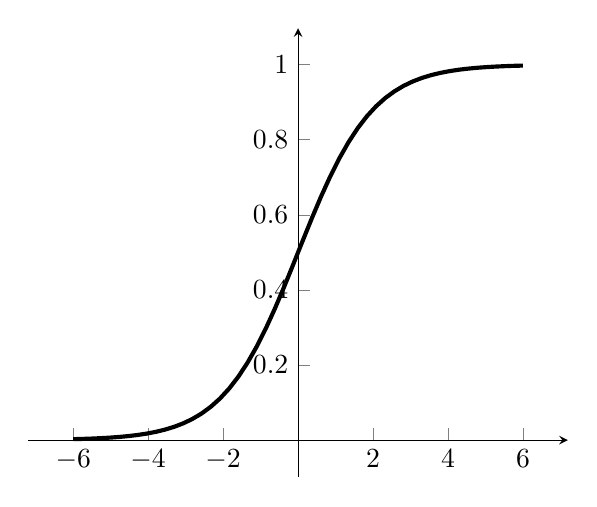
\begin{tikzpicture}
                \begin{axis}[
                  axis lines=center,
                  enlargelimits,
                  tick align=inside,
                  domain=-6:6,
                  samples=50,
                ]
                  \addplot +[mark=none, line width=1.5, color=black] {1/(1+e^(-\x))};
                \end{axis}
              \end{tikzpicture}
            }
            \caption{%
              Plot of the $\sigma_{1, 1}(x)$ function.
            }
          \end{figure}

          Note: calculating the derivative involves a few tricks. First the
          function is rewritten using the fact that for all
          $\beta \in \mathbb{R}$, the $e^{\beta \cdot x} > 0$ inequality holds:

          \begin{align*}
            \sigma_{\beta, \gamma} (x)
              = \frac{\gamma}{1 + e^{- \beta \cdot x}}
              = \frac{\gamma}{1 + \frac{1}{e^{\beta \cdot x}}}
              = \frac{\gamma}{1 + \frac{1}{e^{\beta \cdot x}}} \cdot 1
              = \frac{\gamma}{1 + \frac{1}{e^{\beta \cdot x}}}
                \cdot
                \frac{e^{\beta \cdot x}}{e^{\beta \cdot x}}
              = \frac{\gamma \cdot e^{\beta \cdot x}}{e^{\beta \cdot x} + 1}
          \end{align*}

          Then the derivative:

          \begin{align*}
            \sigma_{\beta, \gamma}' (x)
              & = \frac{
                    \left( \gamma \cdot e^{\beta \cdot x} \right)'
                    \cdot
                    \left(e^{\beta \cdot x} + 1 \right)
                    -
                    \gamma
                    \cdot
                    e^{\beta \cdot x}
                    \cdot
                    \left(e^{\beta \cdot x} + 1 \right)'
                  }{
                    \left(e^{\beta \cdot x} + 1 \right)^2
                  } \\
              & = \frac{
                    \left( \gamma \cdot \beta \cdot e^{\beta \cdot x} \right)
                    \cdot
                    \left(e^{\beta \cdot x} + 1 \right)
                    -
                    \gamma
                    \cdot
                    e^{\beta \cdot x}
                    \cdot
                    \left( \beta \cdot e^{\beta \cdot x} \right)
                  }{
                    \left(e^{\beta \cdot x} + 1 \right)^2
                  } \\
              & = \frac{
                    \gamma \cdot \beta \cdot e^{2 \cdot \beta \cdot x}
                    +
                    \gamma \cdot \beta \cdot e^{\beta \cdot x}
                    -
                    \gamma \cdot \beta \cdot e^{2 \cdot \beta \cdot x}
                  }{
                    \left(e^{\beta \cdot x} + 1 \right)^2
                  } \\
              & = \frac{
                    \gamma \cdot \beta \cdot e^{\beta \cdot x}
                  }{
                    \left(e^{\beta \cdot x} + 1 \right)^2
                  } \\
              & = \frac{
                    \gamma \cdot \beta \cdot e^{\beta \cdot x}
                  }{
                    e^{\beta \cdot x} + 1
                  }
                  \cdot
                  \frac{1}{e^{\beta \cdot x} + 1} \\
              & = \frac{
                    \gamma \cdot \beta \cdot e^{\beta \cdot x}
                  }{
                    e^{\beta \cdot x} + 1
                  }
                  \cdot
                  \frac{
                    e^{\beta \cdot x} + 1 - e^{\beta \cdot x}
                  }{
                    e^{\beta \cdot x} + 1
                  } \\
              & = \frac{
                    \gamma \cdot \beta \cdot e^{\beta \cdot x}
                  }{
                    e^{\beta \cdot x} + 1
                  }
                  \cdot
                  \left(
                    \frac{e^{\beta \cdot x} + 1}{e^{\beta \cdot x} + 1}
                    -
                    \frac{e^{\beta \cdot x}}{e^{\beta \cdot x} + 1}
                  \right) \\
              & = \frac{
                    \gamma \cdot \beta \cdot e^{\beta \cdot x}
                  }{
                    e^{\beta \cdot x} + 1
                  }
                  \cdot
                  \left(
                    1 - \frac{e^{\beta \cdot x}}{e^{\beta \cdot x} + 1}
                  \right) \\
              & = \beta \cdot \sigma_{\beta, \gamma} (x)
                  \cdot
                  \left(
                    1 - \frac{1}{\gamma} \cdot \sigma_{\beta, \gamma} (x)
                  \right) \\
          \end{align*}

        \paragraph{ReLU function}

          Rectified Linear Unit.

          \begin{align*}
            \text{ReLU} (x) = \max(0, x)
            & \quad &
            \text{ReLU}' (x) =
              \begin{cases}
                1 & \text{ if } x > 0 \\
                0 & \text{ if } x < 0
              \end{cases}
          \end{align*}

          Note: $\text{ReLU}(x)$ is not differentiable at $x=0$, but when
          implementing a neural network, people just arbitrarily choose the
          value of $\text{ReLU}'(0)$ to be either $0$ or $1$.

          \begin{figure}[!htb]
            \centering
            \resizebox{!}{0.57\height}{
              \begin{tikzpicture}
                \begin{axis}[
                  axis lines=center,
                  enlargelimits,
                  tick align=inside,
                  domain=-6:6,
                  samples=50,
                ]
                  \addplot +[mark=none, line width=1.5, color=black, domain=-6:0] (x, 0);
                  \addplot +[mark=none, line width=1.5, color=black, domain=0:6] {\x};
                \end{axis}
              \end{tikzpicture}
            }
            \caption{%
              Plot of the $\text{ReLu}(x)$ function.
            }
          \end{figure}

        \paragraph{Parametric ReLU function}

          \begin{align*}
            \text{PReLU}_\beta (x) =
              \begin{cases}
                x & \text{ if } x > 0 \\
                \beta \cdot x & \text{ if } x \leq 0
              \end{cases}
            & \quad &
            \text{PReLU}_\beta' (x) =
              \begin{cases}
                1 & \text{ if } x > 0 \\
                \beta & \text{ if } x < 0
              \end{cases}
          \end{align*}

          \begin{figure}[!htb]
            \centering
            \resizebox{!}{0.57\height}{
              \begin{tikzpicture}
                \begin{axis}[
                  axis lines=center,
                  enlargelimits,
                  tick align=inside,
                  domain=-6:6,
                  samples=6,
                ]
                  \addplot +[mark=none, line width=1.5, color=black, domain=-6:0] {0.05*\x};
                  \addplot +[mark=none, line width=1.5, color=black, domain=0:6] {\x};
                \end{axis}
              \end{tikzpicture}
            }
            \caption{%
              Plot of the $\text{PReLu}_{0.05}(x)$ function.
            }
          \end{figure}

          When $\beta$ is chosen to be a small positive number, e.g. $0.01$,
          then PReLU is also called "leaky ReLU". A leaky ReLU can help
          mitigating the "dying ReLU" problem (a form of the "vanishing gradient
          problem"), which arises when a ReLU neuron is pushed into a state in
          which it becomes inactive for almost all inputs, so the training
          algorithm will no longer be able to get it out from that state.

          Note: $\text{PReLU}(x)$ is not differentiable at $x=0$, but when
          implementing a neural network, people just arbitrarily chose the value
          of $\text{PReLU}'(0)$ to be either $\beta$ or $1$.

        \paragraph{SiLU function}

          Sigmoid Linear Unit, also known as Swish function.

          \begin{align*}
            \text{SiLU}_{\beta, \gamma} (x) = x \cdot \sigma_{\beta, \gamma}(x)
            & \quad &
            \text{SiLU}_{\beta, \gamma}' (x)
              = \sigma_{\beta, \gamma}(x)
                \cdot
                \left(
                  1 + x - \frac{1}{\gamma} \cdot \sigma_{\beta, \gamma}(x)
                \right)
          \end{align*}

          \begin{figure}[!htb]
            \centering
            \resizebox{!}{0.57\height}{
              \begin{tikzpicture}
                \begin{axis}[
                  axis lines=center,
                  enlargelimits,
                  tick align=inside,
                  domain=-6:6,
                  samples=50,
                ]
                  \addplot +[mark=none, line width=1.5, color=black] {\x/(1+e^(-\x))};
                \end{axis}
              \end{tikzpicture}
            }
            \caption{%
              Plot of the $\text{SiLU}_{1, 1}(x)$ function.
            }
          \end{figure}

        \paragraph{ELU function}

          Exponential Linear Unit. For $0 \leq \beta$:

          \begin{align*}
            \text{ELU}_\beta (x) =
              \begin{cases}
                x & \text{ if } x > 0 \\
                \beta \cdot (e^x - 1) & \text{ if } x \leq 0
              \end{cases}
            & \quad &
            \text{ELU}_\beta' (x) =
              \begin{cases}
                1 & \text{ if } x > 0 \\
                \beta \cdot e^x & \text{ if } x \leq 0
              \end{cases}
          \end{align*}

          Note: strictly speaking, when $\beta \neq 1$, then
          $\text{ELU}_\beta (x)$ is not differentiable at $x=0$.

          \begin{figure}[!htb]
            \centering
            \resizebox{!}{0.57\height}{
              \begin{tikzpicture}
                \begin{axis}[
                  axis lines=center,
                  enlargelimits,
                  tick align=inside,
                  domain=-6:6,
                  samples=50,
                ]
                  \addplot +[mark=none, line width=1.5, color=black, domain=-6:0] {e^\x-1};
                  \addplot +[mark=none, line width=1.5, color=black, domain=0:6] {\x};
                \end{axis}
              \end{tikzpicture}
            }
            \caption{%
              Plot of the $\text{ELU}_{1}(x)$ function.
            }
          \end{figure}

        \paragraph{Softplus function}

          Also known as SmoothReLU function. $\beta$ is called the "sharpness":

          \begin{align*}
            \text{Softplus}_{\beta,\gamma} (x) =
              \frac{\gamma}{\beta} \cdot \ln(1 + e^{\beta \cdot x})
            & \quad &
            \text{Softplus}_{\beta,\gamma}' (x) = \sigma_{\beta, \gamma} (x)
          \end{align*}

          \begin{figure}[!htb]
            \centering
            \resizebox{!}{0.57\height}{
              \begin{tikzpicture}
                \begin{axis}[
                  axis lines=center,
                  enlargelimits,
                  tick align=inside,
                  domain=-6:6,
                  samples=50,
                ]
                  \addplot +[mark=none, line width=1.5, color=black] {ln(1+e^\x)};
                \end{axis}
              \end{tikzpicture}
            }
            \caption{%
              Plot of the $\text{Softplus}_{1,1}(x)$ function.
            }
          \end{figure}

        \paragraph{Mish function}

          \begin{align*}
            \text{Mish}_\beta (x)
              & = x \cdot \tanh(\text{Softplus}_{\beta, 1} (x)) \\
            \text{Mish}_\beta' (x)
              & = \tanh(\text{Softplus}_{\beta, 1} (x))
                  +
                  x
                  \cdot
                  \sigma_{\beta, 1} (x)
                  \cdot
                  \text{sech}^2 \left( \text{Softplus}_{\beta, 1} (x) \right)
          \end{align*}

          Where the $\tanh : \mathbb{R} \rightarrow \mathbb{R}$ and the
          $\text{sech} : \mathbb{R} \rightarrow \mathbb{R}$ functions can be
          defined as:

          \begin{align*}
            \tanh(x) = \frac{e^{2 \cdot x} -1}{e^{2 \cdot x} + 1}
            & \quad &
            \text{sech} (x) = \frac{2}{e^x + e^{-x}}
          \end{align*}

          \begin{figure}[!htb]
            \centering
            \resizebox{!}{0.57\height}{
              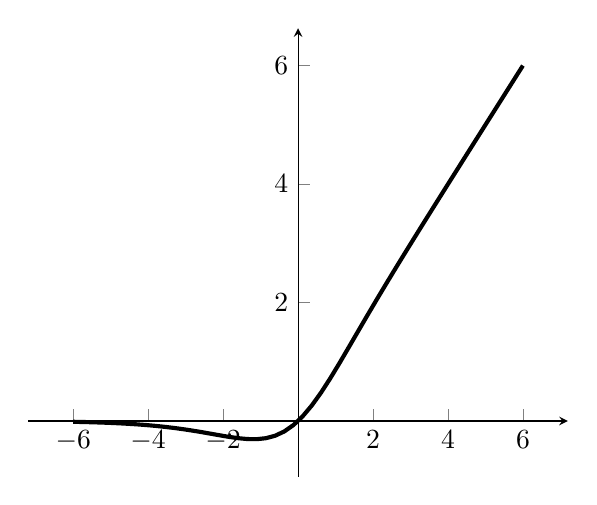
\begin{tikzpicture}
                \begin{axis}[
                  axis lines=center,
                  enlargelimits,
                  tick align=inside,
                  domain=-6:6,
                  samples=50,
                ]
                  \addplot +[mark=none, line width=1.5, color=black] {\x * tanh(ln(1+e^\x))};
                \end{axis}
              \end{tikzpicture}
            }
            \caption{%
              Plot of the $\text{Mish}_{1}(x)$ function.
            }
          \end{figure}

        \paragraph{Squareplus function}

          For $0 \leq \beta$:

          \begin{align*}
            \text{Squareplus}_{\beta} (x) = \frac{x + \sqrt{x^2 + \beta}}{2}
            & \quad &
            \text{Squareplus}_{\beta}' (x)
              = \frac{1}{2} + \frac{x}{2 \cdot \sqrt{x^2 + \beta}}
          \end{align*}

          \begin{figure}[!htb]
            \centering
            \resizebox{!}{0.57\height}{
              \begin{tikzpicture}
                \begin{axis}[
                  axis lines=center,
                  enlargelimits,
                  tick align=inside,
                  domain=-6:6,
                  samples=50,
                ]
                  \addplot +[mark=none, line width=1.5, color=black] {(\x+sqrt(\x^2+1))/2};
                \end{axis}
              \end{tikzpicture}
            }
            \caption{%
              Plot of the $\text{Squareplus}_{1}(x)$ function.
            }
          \end{figure}

\newpage

    \subsection{Neural network}

      Neurons are arranged in layers, the activations of the neurons in a layer
      are the inputs of the next layer.

      Let $L \in \mathbb{N}^+$ denote the number of non-input layers in a
      neural network.

      Let $\mathbf{n} \in \left( {\mathbb{N}^+} \right)^L$ denote the number of
      neurons in each layer of the network, and let $n_0 \in \mathbb{N}^+$
      denote the number of input neurons (features).

      For $L \geq k \in \mathbb{N}$, the $\mathbf{a}^{(k)} \in
      \mathbb{R}^{n_k}$ vector represents the activations in the $k$-th layer;
      $\mathbf{a}^{(0)}$ is the input layer, $\mathbf{a}^{(L)}$ is the output
      layer. Layers between the input and the output layer are called "hidden
      layers". (The parenthesized superscript here is used for indexing the
      layers, and not for powers.)

      The interpretation of the output layer depends on the problem that the
      network is supposed to solve, and it may require extensive experimentation
      to see what works best. For example, a network that recognizes
      handwritten digits may produce its output in a signle neuron, where a
      value in the $[0, 0.1]$ interval means $0$, a value in the $(0.1, 0.2]$
      interval means $1$, and so on, or it could produce its output in 10
      different neurons where the first one shows how much probability the
      network assigns to the input image being a handwritten $0$, the second one
      showing the probability of a handwritten $1$, and so on. (There could even
      be an 11th neuron which signals an unrecognized character.)

      \begin{figure}[!htb]
        \centering
        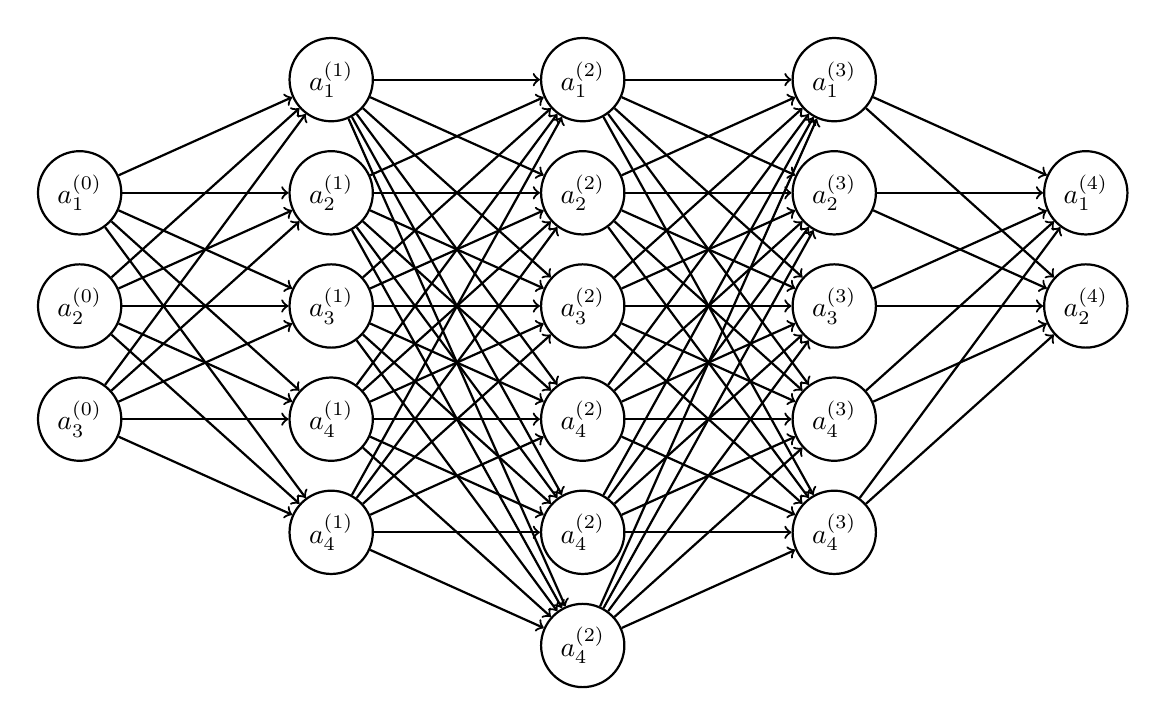
\begin{tikzpicture}[
          neuron/.style={
            circle,
            thick,
            draw=black,
          },
        ]
          \matrix[row sep=1em, column sep=6em]{%
            & \node[neuron](n11){$a_1^{(1)}$};
              & \node[neuron](n21){$a_1^{(2)}$};
              & \node[neuron](n31){$a_1^{(3)}$};
              & \\

            \node[neuron](i1){$a_1^{(0)}$};
              & \node[neuron](n12){$a_2^{(1)}$};
              & \node[neuron](n22){$a_2^{(2)}$};
              & \node[neuron](n32){$a_2^{(3)}$};
              & \node[neuron](o1){$a_1^{(4)}$}; \\

            \node[neuron](i2){$a_2^{(0)}$};
              & \node[neuron](n13){$a_3^{(1)}$};
              & \node[neuron](n23){$a_3^{(2)}$};
              & \node[neuron](n33){$a_3^{(3)}$};
              & \node[neuron](o2){$a_2^{(4)}$}; \\

            \node[neuron](i3){$a_3^{(0)}$};
              & \node[neuron](n14){$a_4^{(1)}$};
              & \node[neuron](n24){$a_4^{(2)}$};
              & \node[neuron](n34){$a_4^{(3)}$};
              & \\

            & \node[neuron](n15){$a_4^{(1)}$};
              & \node[neuron](n25){$a_4^{(2)}$};
              & \node[neuron](n35){$a_4^{(3)}$};
              & \\

            & & \node[neuron](n26){$a_4^{(2)}$}; & & \\
          };
          \draw
              (i1) edge [->,thick] (n11)
              (i1) edge [->,thick] (n12)
              (i1) edge [->,thick] (n13)
              (i1) edge [->,thick] (n14)
              (i1) edge [->,thick] (n15)

              (i2) edge [->,thick] (n11)
              (i2) edge [->,thick] (n12)
              (i2) edge [->,thick] (n13)
              (i2) edge [->,thick] (n14)
              (i2) edge [->,thick] (n15)

              (i3) edge [->,thick] (n11)
              (i3) edge [->,thick] (n12)
              (i3) edge [->,thick] (n13)
              (i3) edge [->,thick] (n14)
              (i3) edge [->,thick] (n15)

              (n11) edge [->,thick] (n21)
              (n11) edge [->,thick] (n22)
              (n11) edge [->,thick] (n23)
              (n11) edge [->,thick] (n24)
              (n11) edge [->,thick] (n25)
              (n11) edge [->,thick] (n26)

              (n12) edge [->,thick] (n21)
              (n12) edge [->,thick] (n22)
              (n12) edge [->,thick] (n23)
              (n12) edge [->,thick] (n24)
              (n12) edge [->,thick] (n25)
              (n12) edge [->,thick] (n26)

              (n13) edge [->,thick] (n21)
              (n13) edge [->,thick] (n22)
              (n13) edge [->,thick] (n23)
              (n13) edge [->,thick] (n24)
              (n13) edge [->,thick] (n25)
              (n13) edge [->,thick] (n26)

              (n14) edge [->,thick] (n21)
              (n14) edge [->,thick] (n22)
              (n14) edge [->,thick] (n23)
              (n14) edge [->,thick] (n24)
              (n14) edge [->,thick] (n25)
              (n14) edge [->,thick] (n26)

              (n15) edge [->,thick] (n21)
              (n15) edge [->,thick] (n22)
              (n15) edge [->,thick] (n23)
              (n15) edge [->,thick] (n24)
              (n15) edge [->,thick] (n25)
              (n15) edge [->,thick] (n26)

              (n21) edge [->,thick] (n31)
              (n21) edge [->,thick] (n32)
              (n21) edge [->,thick] (n33)
              (n21) edge [->,thick] (n34)
              (n21) edge [->,thick] (n35)

              (n22) edge [->,thick] (n31)
              (n22) edge [->,thick] (n32)
              (n22) edge [->,thick] (n33)
              (n22) edge [->,thick] (n34)
              (n22) edge [->,thick] (n35)

              (n23) edge [->,thick] (n31)
              (n23) edge [->,thick] (n32)
              (n23) edge [->,thick] (n33)
              (n23) edge [->,thick] (n34)
              (n23) edge [->,thick] (n35)

              (n24) edge [->,thick] (n31)
              (n24) edge [->,thick] (n32)
              (n24) edge [->,thick] (n33)
              (n24) edge [->,thick] (n34)
              (n24) edge [->,thick] (n35)

              (n25) edge [->,thick] (n31)
              (n25) edge [->,thick] (n32)
              (n25) edge [->,thick] (n33)
              (n25) edge [->,thick] (n34)
              (n25) edge [->,thick] (n35)

              (n26) edge [->,thick] (n31)
              (n26) edge [->,thick] (n32)
              (n26) edge [->,thick] (n33)
              (n26) edge [->,thick] (n34)
              (n26) edge [->,thick] (n35)

              (n31) edge [->,thick] (o1)
              (n31) edge [->,thick] (o2)

              (n32) edge [->,thick] (o1)
              (n32) edge [->,thick] (o2)

              (n33) edge [->,thick] (o1)
              (n33) edge [->,thick] (o2)

              (n34) edge [->,thick] (o1)
              (n34) edge [->,thick] (o2)

              (n35) edge [->,thick] (o1)
              (n35) edge [->,thick] (o2);
        \end{tikzpicture}
        \caption{%
          A neural network with 3 input neurons, 3 hidden layers, and 2 output
          neurons.
        }
      \end{figure}

      For $L \geq k \in \mathbb{N}^+$, the
      $\mathbf{W}^{(k)} \in \mathbb{R}^{n_{k} \times n_{k-1}}$ matrix represents
      the weights of the connections from the $k-1$-th layer to the $k$-th
      layer, and the $\mathbf{b}^{(k)} \in \mathbb{R}^{n_k}$ vector represents
      the biases in the $k$-th layer.

      Let $\mathbf{f}^{(k)} ( \mathbf{x} )$ for
      $\mathbf{x} \in \mathbb{R}^{n_k}$ denote the
      $\left[ f_j^{(k)} ( x_j ) \right]_{j=1}^{n_k} \in \mathbb{R}^{n_k}$ vector
      where $f_j^{(k)} : \mathbb{R} \rightarrow \mathbb{R}$ is the function
      that is used for calculating the activation of the $j$-th neuron in the
      $k$-th layer.

      The activation of the $k$-th layer (where $L \geq k \in \mathbb{N}^+$)
      can be calculated as:

      \begin{equation}\label{eqactivation}
        \mathbf{a}^{(k)} =
          \mathbf{f}^{(k)} \left(
            \mathbf{W}^{(k)} \cdot \mathbf{a}^{(k-1)} + \mathbf{b}^{(k)}
          \right)
      \end{equation}

      \subsubsection{Simplified notation}\label{simplifiednotation}

        For $L \geq k \in \mathbb{N}$, let $a_0^{(k)} = 1$, and if $k > 0$ then
        for $n_k \geq j \in \mathbb{N}^+$, let $w_{j, 0}^{(k)} = b_{j}^{(k)}$,
        and for $n_{k-1} \geq i \in \mathbb{N}$, let $w_{0,i} = 1$,
        and let $f_0^{(k)} = \text{id}$, and let $w_{0,0}=0$.

        With this notation, equation \ref{eqactivation} can be simplified:

        \begin{equation}\label{eqactivationsimple}
          \mathbf{a}^{(k)} =
            \mathbf{f}^{(k)} \left(
              \mathbf{W}^{(k)} \cdot \mathbf{a}^{(k-1)}
            \right)
        \end{equation}

      \subsubsection{Examples}

        \paragraph{Feed-forward network}

          A network with no loops (backward connections).

        \paragraph{Recurrent network}

          A network with loops (backward connections).

        \paragraph{Perceptron}

          A single layer, single output ($L = 1, n_1 = 1$) feed-forward network.

          \subparagraph{Majority function perceptron}

            Tells if more than half ofits inputs are 1.

            $w_{1,j} = 1$ ($n_0 \geq j \in \mathbb{N}^+$) and
            $b_1 = \frac{n_0}{2}$.

          \subparagraph{Linear separator}
            With the simplified notation (\ref {simplifiednotation}), the
            activation of the perceptron can be written as:

            \begin{equation}
              a^{(1)} = f \left( \mathbf{W}^{(1)} \cdot \mathbf{a}^{(0)} \right)
            \end{equation}

            Since the $\mathbf{W}^{(1)} \cdot \mathbf{a}^{(0)} = 0$ equation
            defines a hyperplane in $n_0$ dimensions, a perceptron with $f$
            being the threshold function (\ref{eqthreshold}) can be thought
            of as a classifier which separates inputs that lie on one side of
            the plane from the inputs that lie on the other side.

            A binary function ($f : \mathbb{R}^n \rightarrow \{0, 1\}$ for some
            $n \in \mathbb{N}^+$) is linearly separable if its inputs that yield
            $1$ can be separated from the inputs which yield $0$ with a
            straight line (or plane, or hyperplane). For example, the
            $\text{OR}, \text{AND} : \{ 0, 1 \}^2 \rightarrow \{ 0, 1 \}$
            functions are linearly separable:

            \begin{eqnarray*}
              \text{OR}(x, y) & = & \begin{cases}
                  0 & \text{ if } x = y = 0 \\
                  1 & \text{ otherwise }
                \end{cases} \\
              \text{AND}(x, y) & = & \begin{cases}
                  1 & \text{ if } x = y = 1 \\
                  0 & \text{ otherwise}
                \end{cases}
            \end{eqnarray*}

            But the $\text{XOR} : \{ 0, 1 \}^2 \rightarrow \{ 0, 1 \}$ function
            is not linearly separable:

            \begin{equation*}
              \text{XOR}(x, y) = \begin{cases}
                  1 & \text{ if } (x, y) \in \{ (0, 1), (1, 0) \} \\
                  0 & \text{ otherwise}
                \end{cases}
            \end{equation*}

            Note that a function which is not linearly separable in
            $n \in \mathbb{N}^+$ dimensions may be turned into a linearly
            separable function by cleverly adding extra dimensions.

\newpage

  \section{Learning, gradient descent, backpropagation}

    All the weights and biases are initialized with random values. The
    activation of the output layer is then calculated for a number of example
    inputs for which the desired output is already known (supervised learning),
    and the weights and biases are adjusted so that the average difference
    between the calculated and the desired outputs is minimized.

    The idea is to define an error function in terms of the weights and biases
    in the network, treating the input activations like constants. If all the
    activation functions are differentiable, then this error function is also
    differentiable, so its gradient for a given set of weigths and biases will
    give the direction and the rate of the fastest increase. Since the goal is
    to minimize the error, we will multiply the gradient by $-1$ to get the
    direction of the fastest decrease, and use that to adjust the weights and
    biases for each example input. As more and more adjustments are made for
    more and more examples, the error function should converge towards a
    (local) minimum and thus, its gradient should converge towards $0$. (Hence
    the name "gradient descent".) Making the step size at each iteration
    proportional to the length of the gradient vector can help avoiding
    overshooting.

    (From now on, the differentiability of $f_j^{(k)}$ is assumed for all
    $j, k \in \mathbb{N}^+, k \leq L, j \leq n_k$.)

    \subsection{Error function}

      (Also known as Cost function.)

      Let $\mathbf{y} \in \mathbb{R}^{n_L}$ denote the expected output
      activations for a given $\mathbf{a}^{(0)} \in \mathbb{R}^{n_0}$ example
      input. One way to define an error function for this single example input
      is the following (where $C : \mathbb{R}^{n_0} \rightarrow \mathbb{R}$):

      \begin{equation}\label{eqerror}
        \begin{split}
          C \left( \mathbf{a}^{(0)} \right)
              & = \frac{1}{2}
                  \cdot
                  \left\|
                    \mathbf{a}^{(L)} - \mathbf{y}
                  \right\|_2^{\enspace 2} \\
              & = \frac{1}{2}
                  \cdot
                  \left(
                    \sqrt{
                      \sum_{j=1}^{n_L} \left( a_j^{(L)} - y_j \right)^2
                    }
                  \right)^2
                = \frac{1}{2}
                  \cdot
                  \sum_{j=1}^{n_L} \left( a_j^{(L)} - y_j \right)^2 \\
              & = \sum_{j=1}^{n_L}
                    \frac{1}{2} \cdot \left( a_j^{(L)} - y_j \right)^2
        \end{split}
      \end{equation}

      \subsubsection{Gradient}

        To find $\nabla C$, we need the partial derivatives for each
        $w_{u^{(k)},v^{(k-1)}}^{(k)}$
        (for $
          k, u^{(k)}, v^{(k-1)} \in \mathbb{N},
          1 \leq k \leq L,
          1 \leq u^{(k)} \leq n_k,
          v^{(k-1)} \leq n_{k-1}
        $).

        \paragraph{Notation}

          \subparagraph{$\Delta_j^{(k)}$}

            For a given $L \geq k \in \mathbb{N}^+$ and
            $n_k \geq j \in \mathbb{N}$ and
            $\mathbf{a}^{(0)} \in \mathbb{R}^{n_0}$, let

            \begin{equation}
              \Delta_j^{(k)}
                = {f_j^{(k)}}' \left(
                    \sum_{i=0}^{n_{k-1}} w_{j,i}^{(k)} \cdot a_i^{(k-1)}
                  \right)
            \end{equation}

            and

            \begin{equation}
              \mathbf{\Delta}^{(k)}
                = \left[ \Delta_j^{(k)} \right]_{j=0}^{n_k}
                = \begin{bmatrix}
                    \vspace{1.5ex}
                    \Delta_0^{(k)} \\
                    \vspace{1.5ex}
                    \Delta_1^{(k)} \\
                    \Delta_2^{(k)} \\
                    \vdots \\
                    \Delta_{n_k}^{(k)}
                  \end{bmatrix}
            \end{equation}

            Note:

            \begin{equation}
              \Delta_0^{(k)}
                = {f_0^{(k)}}' \left(
                    \sum_{i=0}^{n_{k-1}} w_{j,i}^{(k)} \cdot a_i^{(k-1)}
                  \right)
                = {\text{id}}' \left(
                    \sum_{i=0}^{n_{k-1}} w_{0,i}^{(k)} \cdot a_i^{(k-1)}
                  \right)
                = 1
            \end{equation}

          \subparagraph{${\mathbf{f}^{(k)}}'(\mathbf{x})$}

            For a given $L \geq k \in \mathbb{N}^+$ and
            $\mathbf{x} \in \mathbb{R}^{n_k}$:

              \begin{equation}
                {\mathbf{f}^{(k)}}'(\mathbf{x})
                  = \left[ {f_j^{(k)}}' \left( x_j \right) \right]_{j=0}^{n_k}
                  = \begin{bmatrix}
                      \vspace{1.5ex}
                      {f_0^{(k)}}' \left( x_0 \right) \\
                      \vspace{1.5ex}
                      {f_1^{(k)}}' \left( x_1 \right) \\
                      {f_2^{(k)}}' \left( x_2 \right) \\
                      \vdots \\
                      {f_{n_k}^{(k)}}' \left( x_{n_k} \right)
                    \end{bmatrix}
              \end{equation}

        \paragraph{Output layer}

          Partial derivatives using equation \ref{eqerror}
          ($u, v \in \mathbb{N}, 1 \leq u \leq n_L, v \leq n_{L-1}$):

          \begin{equation}
            \begin{split}
              \frac{\partial}{\partial w_{u,v}^{(L)}}
                C \left( \mathbf{a}^{(0)} \right)
                  = & \frac{\partial}{\partial w_{u,v}^{(L)}}
                        \sum_{j=1}^{n_L}
                          \frac{1}{2} \cdot \left( a_j^{(L)} - y_j \right)^2 \\
                  = & \sum_{j=1}^{n_L}
                        \frac{1}{2}
                        \cdot
                        \frac{\partial}{\partial w_{u,v}^{(L)}}
                          \left( a_j^{(L)} - y_j \right)^2 \\
                  = & \sum_{j=1}^{n_L}
                        \frac{1}{2}
                        \cdot
                        \frac{\partial}{\partial w_{u,v}^{(L)}}
                          \left(
                            f_j^{(L)} \left(
                              \sum_{i=0}^{n_{L-1}}
                                w_{j,i}^{(L)} \cdot a_{i}^{(L-1)}
                            \right)
                            - y_j
                          \right)^2
            \end{split}
          \end{equation}

          Since most of the terms in the outer summation don't depend on
          $w_{u,v}^{(L)}$, they can be treated as constants, and therefore their
          derivative is 0, and the only one that remains is  where $j=u$:

          \begin{equation}
            \frac{\partial}{\partial w_{u,v}^{(L)}}
              C \left( \mathbf{a}^{(0)} \right)
                = \frac{1}{2}
                  \cdot
                  \frac{\partial}{\partial w_{u,v}^{(L)}}
                    \left(
                      f_{u}^{(L)} \left(
                        \sum_{i=0}^{n_{L-1}} w_{u,i}^{(L)} \cdot a_{i}^{(L-1)}
                      \right)
                      - y_{u}
                    \right)^2
          \end{equation}

          Applying the chain rule (note that the $a_i^{(L-1)}$ terms don't
          depend on $w_{u,v}^{(L)}$ either):

          \begin{equation}
            \begin{split}
              \frac{\partial}{\partial w_{u,v}^{(L)}}
                C \left( \mathbf{a}^{(0)} \right)
                  = & \frac{1}{2}
                      \cdot
                      2
                      \cdot
                      \left(
                          f_{u}^{(L)} \left(
                            \sum_{i=0}^{n_{L-1}}
                              w_{u,i}^{(L)} \cdot a_{i}^{(L-1)}
                          \right)
                          - y_{u}
                        \right)
                      \cdot
                        {f_{u}^{(L)}}' \left(
                          \sum_{i=0}^{n_{L-1}}
                            w_{u,i}^{(L)} \cdot a_{i}^{(L-1)}
                        \right)
                      \cdot
                        a_{v}^{(L-1)}
            \end{split}
          \end{equation}

          Rearranging and shortening:

          \begin{equation}
            \frac{\partial}{\partial w_{u,v}^{(L)}}
              C \left( \mathbf{a}^{(0)} \right)
                = \left( a_{u}^{(L)} - y_{u} \right)
                  \cdot
                  \Delta_u^{(L)}
                  \cdot
                  a_{v}^{(L-1)}
          \end{equation}

        \paragraph{Last hidden layer}

          Partial derivatives for the $L - 1$-th layer if $L \geq 2$,
          for $u, v \in \mathbb{N}, 1 \leq u \leq n_{L-1}, v \leq n_{L-2}$,
          using equation \ref{eqerror}:

          \begin{equation}\label{eqlasthittenpartder0}
            \begin{split}
              \frac{\partial}{\partial w_{u,v}^{(L-1)}}
                C \left( \mathbf{a}^{(0)} \right)
                  = & \frac{\partial}{\partial w_{u,v}^{(L-1)}}
                        \sum_{j=1}^{n_L}
                          \frac{1}{2}
                          \cdot
                          \left( a_j^{(L)} - y_j \right)^2 \\
                  = & \sum_{j=1}^{n_L}
                        \frac{1}{2}
                        \cdot
                        \frac{\partial}{\partial w_{u,v}^{(L-1)}}
                          \left( a_j^{(L)} - y_j \right)^2
            \end{split}
          \end{equation}

          Now all of the terms inside the summation depend on
          $w_{u,v}^{(L-1)}$, because $a_j^{(L)}$ depends on it for
          all $n_L \geq j \in \mathbb{N}+$.

          Using the chain rule, expanding $a_j^{(L)}$ for a given
          $n_L \geq j \in \mathbb{N}^+$, and exploiting the fact that none of
          the weights and biases in the output layer depend on the weights and
          biases in the last hidden layer:

          \begin{equation}\label{eqlasthittenpartder1}
            \begin{split}
              \frac{1}{2}
              \cdot
              \frac{\partial}{\partial w_{u,v}^{(L-1)}}
                \left( a_j^{(L)} - y_j \right)^2
                & = \frac{1}{2}
                    \cdot
                    2
                    \cdot
                    \left( a_j^{(L)} - y_j \right)
                    \cdot
                    \frac{\partial}{\partial w_{u,v}^{(L-1)}}
                      a_j^{(L)} \\
                & = \left( a_j^{(L)} - y_j \right)
                    \cdot
                    \frac{\partial}{\partial w_{u,v}^{(L-1)}}
                      f_j^{(L)} \left(
                        \sum_{i=0}^{n_{L-1}} w_{j,i}^{(L)} \cdot a_i^{(L-1)}
                      \right) \\
                & = \left( a_j^{(L)} - y_j \right)
                    \cdot
                    {f_j^{(L)}}' \left(
                      \sum_{i=0}^{n_{L-1}} w_{j,i}^{(L)} \cdot a_i^{(L-1)}
                    \right)
                    \cdot
                    \frac{\partial}{\partial w_{u,v}^{(L-1)}}
                      \left(
                        \sum_{i=0}^{n_{L-1}} w_{j,i}^{(L)} \cdot a_i^{(L-1)}
                      \right) \\
                & = \left( a_j^{(L)} - y_j \right)
                    \cdot
                    \Delta_j^{(L)}
                    \cdot
                    \left(
                      \sum_{i=0}^{n_{L-1}}
                        w_{j,i}^{(L)}
                        \cdot
                        \frac{\partial}{\partial w_{u,v}^{(L-1)}}
                          a_i^{(L-1)}
                    \right)
            \end{split}
          \end{equation}

          Since only $a_{u}^{(L-1)}$ depends on $w_{u,v}^{(L-1)}$, most of the
          terms in the summation are $0$ (because they are multiplied by the
          derivative of a constant, which is $0$), and the only one that remains
          is where $i = u$. Continuing equation \ref{eqlasthittenpartder1}:

          \begin{equation}\label{eqlasthittenpartder2}
            \frac{1}{2}
            \cdot
            \frac{\partial}{\partial w_{u,v}^{(L-1)}}
              \left( a_j^{(L)} - y_j \right)^2
                = \left( a_j^{(L)} - y_j \right)
                  \cdot
                  \Delta_j^{(L)}
                  \cdot
                  w_{j,u}^{(L)}
                  \cdot
                  \frac{\partial}{\partial w_{u,v}^{(L-1)}}
                    a_{u}^{(L-1)}
          \end{equation}

          Expanding $a_{u}^{(L-1)}$, and using the chain rule again:

          \begin{equation}\label{eqlasthittenpartder3}
            \begin{split}
              \frac{\partial}{\partial w_{u,v}^{(L-1)}}
                a_{u}^{(L-1)}
                  = & \frac{\partial}{\partial w_{u,v}^{(L-1)}}
                      f_{u}^{(L-1)} \left(
                        \sum_{m=0}^{n_{L-2}}
                          w_{u,m}^{(L-1)} \cdot a_m^{(L-2)}
                      \right) \\
                  = & {f_{u}^{(L-1)}}' \left(
                        \sum_{m=0}^{n_{L-2}}
                          w_{u,m}^{(L-1)} \cdot a_m^{(L-2)}
                      \right)
                      \cdot
                      \frac{\partial}{\partial w_{u,v}^{(L-1)}}
                        \left(
                          \sum_{m=0}^{n_{L-2}}
                            w_{u,m}^{(L-1)} \cdot a_m^{(L-2)}
                        \right) \\
                  = & \Delta_u^{(L-1)}
                      \cdot
                      \left(
                        \sum_{m=0}^{n_{L-2}}
                          \frac{\partial}{\partial w_{u,v}^{(L-1)}}
                            w_{u,m}^{(L-1)} \cdot a_m^{(L-2)}
                      \right)
            \end{split}
          \end{equation}

          Since only one term in the summation depends on $w_{u,v}^{(L-1)}$
          (the one where $m = v$), most of the terms are $0$, because they are
          multiplied by the derivative of a constant, which is $0$. Continuing
          equation \ref{eqlasthittenpartder3}:

          \begin{equation}
            \frac{\partial}{\partial w_{u,v}^{(L-1)}}
              a_{u}^{(L-1)}
                = \Delta_u^{(L-1)}
                  \cdot
                  \frac{\partial}{\partial w_{u,v}^{(L-1)}}
                    w_{u,v}^{(L-1)} \cdot a_{v}^{(L-2)}
                = \Delta_u^{(L-1)} \cdot a_{v}^{(L-2)}
          \end{equation}

          Plugging this back into equation \ref{eqlasthittenpartder2} and then
          that into equation \ref{eqlasthittenpartder0}:

          \begin{equation}
            \frac{\partial}{\partial w_{u,v}^{(L-1)}}
              C \left( \mathbf{a}^{(0)} \right)
                = \sum_{j=1}^{n_L}
                    \left( a_j^{(L)} - y_j \right)
                    \cdot
                    \Delta_j^{(L)}
                    \cdot
                    w_{j,u}^{(L)}
                    \cdot
                    \Delta_u^{(L-1)}
                    \cdot
                    a_{v}^{(L-2)}
          \end{equation}

        \paragraph{In-between hidden layers}

          Partial derivatives for the $k$-th layer for $L \geq 3$ and
          $L-2 \geq k \in \mathbb{N}^+$ and
          $u, v \in \mathbb{N}, 1 \leq u \leq n_k, v \leq n_{k - 1}$,
          using equation \ref{eqerror}:

          \begin{equation}\label{eqkthpartder0}
            \begin{split}
              \frac{\partial}{\partial w_{u,v}^{(k)}}
                C \left( \mathbf{a}^{(0)} \right)
                  & = \frac{\partial}{\partial w_{u,v}^{(k)}}
                        \sum_{j=1}^{n_L}
                          \frac{1}{2}
                          \cdot
                          \left( a_j^{(L)} - y_j \right)^2 \\
                  & = \sum_{j=1}^{n_L}
                        \frac{1}{2}
                        \cdot
                        \frac{\partial}{\partial w_{u,v}^{(k)}}
                          \left( a_j^{(L)} - y_j \right)^2 \\
                  & = \sum_{j=1}^{n_L}
                        \frac{1}{2}
                        \cdot
                        2
                        \cdot
                        \left( a_j^{(L)} - y_j \right)
                        \cdot
                        \frac{\partial}{\partial w_{u,v}^{(k)}} a_j^{(L)} \\
                  & = \sum_{j=1}^{n_L}
                        \left( a_j^{(L)} - y_j \right)
                        \cdot
                        \frac{\partial}{\partial w_{u,v}^{(k)}}
                          f_j^{(L)} \left(
                            \sum_{i_1=0}^{n_{L-1}}
                              w_{j,i_1}^{(L)}
                              \cdot
                              a_{i_1}^{(L-1)}
                          \right) \\
                  & = \sum_{j=1}^{n_L}
                        \left( a_j^{(L)} - y_j \right)
                        \cdot
                        \Delta_j^{(L)}
                        \cdot
                        \left(
                          \sum_{i_1=0}^{n_{L-1}}
                            w_{j,i_1}^{(L)}
                            \cdot
                            \frac{\partial}{\partial w_{u,v}^{(k)}}
                              a_{i_1}^{(L-1)}
                        \right) \\
                  & = \sum_{j=1}^{n_L}
                        \left( a_j^{(L)} - y_j \right)
                        \cdot
                        \Delta_j^{(L)}
                        \cdot
                        \left(
                          \sum_{i_1=0}^{n_{L-1}}
                            w_{j,i_1}^{(L)}
                            \cdot
                            \frac{\partial}{\partial w_{u,v}^{(k)}}
                              f_{i_1}^{(L-1)} \left(
                                \sum_{i_2=0}^{n_{L-2}}
                                  w_{i_1,i_2}^{(L-1)}
                                  \cdot
                                  a_{i_2}^{(L-2)}
                              \right)
                        \right) \\
                  & = \sum_{j=1}^{n_L}
                        \left( a_j^{(L)} - y_j \right)
                        \cdot
                        \Delta_j^{(L)}
                        \cdot
                        \left(
                          \sum_{i_1=0}^{n_{L-1}}
                            w_{j,i_1}^{(L)}
                            \cdot
                            \Delta_{i_1}^{(L-1)}
                            \cdot
                            \left(
                              \sum_{i_2=0}^{n_{L-2}}
                                w_{i_1,i_2}^{(L-1)}
                                \cdot
                                \frac{\partial}{\partial w_{u,v}^{(k)}}
                                  a_{i_2}^{(L-2)}
                            \right)
                        \right) \\
                  & = \sum_{j=1}^{n_L}
                        \sum_{i_1=0}^{n_{L-1}}
                          \left( a_j^{(L)} - y_j \right)
                          \cdot
                          \Delta_j^{(L)}
                          \cdot
                          w_{j,i_1}^{(L)}
                          \cdot
                          \Delta_{i_1}^{(L-1)}
                          \cdot
                          \left(
                            \sum_{i_2=0}^{n_{L-2}}
                              w_{i_1,i_2}^{(L-1)}
                              \cdot
                              \frac{\partial}{\partial w_{u,v}^{(k)}}
                                a_{i_2}^{(L-2)}
                          \right) \\
                  & = \sum_{j=1}^{n_L}
                        \sum_{i_1=0}^{n_{L-1}}
                          \sum_{i_2=0}^{n_{L-2}}
                            \left( a_j^{(L)} - y_j \right)
                            \cdot
                            \Delta_j^{(L)}
                            \cdot
                            w_{j,i_1}^{(L)}
                            \cdot
                            \Delta_{i_1}^{(L-1)}
                            \cdot
                            w_{i_1,i_2}^{(L-1)}
                            \cdot
                            \frac{\partial}{\partial w_{u,v}^{(k)}}
                              a_{i_2}^{(L-2)} \\
                  & = \ldots
            \end{split}
          \end{equation}

          Due to the chain rule and the commutativity of addition, the emerging
          pattern of introducing
          $\Delta_{i_{L-l}}^{(l)} \cdot w_{i_{L-l},i_{L-l+1}}^{(l)}$ terms
          (where $l \in \mathbb{N}^+, k < l \leq L$)
          will continue as we go down to deeper and deeper layers, expanding the
          activations. Eventually, we reach the layer immediately above the
          $k$-th layer, where we need to find
          $\frac{\partial}{\partial w_{u,v}^{(k)}} a_{i_{L-(k+1)}}^{(k+1)}$:

          \begin{equation}
            \begin{split}
              \frac{\partial}{\partial w_{u,v}^{(k)}}
                a_{i_{L-(k+1)}}^{(k+1)}
                  & = \frac{\partial}{\partial w_{u,v}^{(k)}}
                        f_{i_{L-(k+1)}}^{(k+1)} \left(
                          \sum_{i_{L-k}=0}^{n_k}
                            w_{i_{L-(k+1)},i_{L-k}}^{(k+1)}
                            \cdot
                            a_{i_{L-k}}^{(k)}
                        \right) \\
                  & = {f_{i_{L-(k+1)}}^{(k+1)}}' \left(
                        \sum_{i_{L-k}=0}^{n_k}
                          w_{i_{L-(k+1)},i_{L-k}}^{(k+1)}
                          \cdot
                          a_{i_{L-k}}^{(k)}
                      \right)
                      \cdot
                      \frac{\partial}{\partial w_{u,v}^{(k)}}
                        \left(
                          \sum_{i_{L-k}=0}^{n_k}
                            w_{i_{L-(k+1)},i_{L-k}}^{(k+1)}
                            \cdot
                            a_{i_{L-k}}^{(k)}
                        \right) \\
                & = \Delta_{i_{L-(k+1)}}^{(k+1)}
                    \cdot
                    \sum_{i_{L-k}=0}^{n_k}
                      w_{i_{L-(k+1)},i_{L-k}}^{(k+1)}
                      \cdot
                      \frac{\partial}{\partial w_{u,v}^{(k)}}
                        a_{i_{L-k}}^{(k)} \\
                & = \Delta_{i_{L-(k+1)}}^{(k+1)}
                    \cdot
                    \sum_{i_{L-k}=0}^{n_k}
                      w_{i_{L-(k+1)},i_{L-k}}^{(k+1)}
                      \cdot
                      \frac{\partial}{\partial w_{u,v}^{(k)}}
                        f_{i_{L-k}}^{(k)} \left(
                          \sum_{i_{L-k+1}=0}^{n_{k-1}}
                            w_{i_{L-k},i_{L-k+1}}^{(k)}
                            \cdot
                            a_{i_{L-k+1}}^{(k-1)}
                        \right) \\
                & = \Delta_{i_{L-(k+1)}}^{(k+1)}
                    \cdot
                    \sum_{i_{L-k}=0}^{n_k}
                      w_{i_{L-(k+1)},i_{L-k}}^{(k+1)}
                      \cdot
                      \Delta_{i_{L-k}}^{(k)}
                      \cdot
                      \frac{\partial}{\partial w_{u,v}^{(k)}}
                        \left(
                          \sum_{i_{L-k+1}=0}^{n_{k-1}}
                            w_{i_{L-k},i_{L-k+1}}^{(k)}
                            \cdot
                            a_{i_{L-k+1}}^{(k-1)}
                        \right) \\
                & = \Delta_{i_{L-(k+1)}}^{(k+1)}
                    \cdot
                    \sum_{i_{L-k}=0}^{n_k}
                      w_{i_{L-(k+1)},i_{L-k}}^{(k+1)}
                      \cdot
                      \Delta_{i_{L-k}}^{(k)}
                      \cdot
                      \left(
                        \sum_{i_{L-k+1}=0}^{n_{k-1}}
                          \frac{\partial}{\partial w_{u,v}^{(k)}}
                            w_{i_{L-k},i_{L-k+1}}^{(k)}
                          \cdot
                          a_{i_{L-k+1}}^{(k-1)}
                      \right)
            \end{split}
          \end{equation}

          The only term which depends on $w_{u,v}^{(k)}$ in the inner summation
          is the one where $i_{L-k} = u$ and $i_{L-k+1} = v$,
          so the derivative of all the other terms is $0$. This also makes the
          terms in the outer summation equal to $0$ where $i_{L-k} \neq u$, so
          we're left with:

          \begin{equation}
            \begin{split}
              \frac{\partial}{\partial w_{u,v}^{(k)}}
                a_{i_{L-(k+1)}}^{(k+1)}
                  & = \Delta_{i_{L-(k+1)}}^{(k+1)}
                      \cdot
                      w_{i_{L-(k+1)},u}^{(k+1)}
                      \cdot
                      \Delta_u^{(k)}
                      \cdot
                      \frac{\partial}{\partial w_{u,v}^{(k)}}
                        w_{u,v}^{(k)}
                      \cdot
                      a_v^{(k-1)} \\
                  & = \Delta_{i_{L-(k+1)}}^{(k+1)}
                      \cdot
                      w_{i_{L-(k+1)},u}^{(k+1)}
                      \cdot
                      \Delta_u^{(k)}
                      \cdot
                      a_v^{(k-1)}
            \end{split}
          \end{equation}

          Therefore the general form of equation \ref{eqkthpartder0} can be
          written as:

          \begin{equation}\label{eqkthpartder1}
            \begin{split}
              \frac{\partial}{\partial w_{u,v}^{(k)}}
                C \left( \mathbf{a}^{(0)} \right)
                    = \sum_{j=1}^{n_L}
                        \sum_{i_1=0}^{n_{L-1}}
                          \ldots
                          \sum_{i_{L-(k+1)}=0}^{n_{k+1}}
                            & \left( a_j^{(L)} - y_j \right) \\
                            & \cdot
                              \Delta_j^{(L)}
                              \cdot
                              w_{j,i_1}^{(L)} \\
                            & \cdot
                              \Delta_{i_1}^{(L-1)}
                              \cdot
                              w_{i_1,i_2}^{(L-1)} \\
                            & \quad \vdots \\
                            & \cdot
                              \Delta_{i_{L-(k+1)}}^{(k+1)}
                              \cdot
                              w_{i_{L-(k+1)},u}^{(k+1)} \\
                            & \cdot
                              \Delta_u^{(k)}
                              \cdot
                              a_v^{(k-1)}
            \end{split}
          \end{equation}

\newpage

    \subsection{Basic backpropagation algorithm}

      As can be seen in equation \ref{eqkthpartder1}, calculating the partial
      derivatives requires an exponentially growing number of additions and
      multiplications as more and more layers are added to a network.
      Fortunately, the values of the
      $
        \left( a_j^{(L)} - y_j \right)
        \cdot
        \Delta_j^{(L)}
        \cdot
        w_{j,i_1}^{(L)}
        \cdot
        \Delta_{i_1}^{(L-1)}
        \cdot
        w_{i_1,i_2}^{(L-1)}
        \cdot
        \ldots
        \Delta_{i_{L-k}}^{(k)}
        \cdot
        w_{i_{L-k},i_{L-k}+1}^{(k)}
      $ products can be cached and reused for subsequent layers if we evaluate
      the activations across the network forward (from the input layer towards
      the output layer), and then calculate the gradient bacwards (from the
      output layer towards the input layer). This backwards propagation of the
      error is where the name of this learning algorithm comes from.

      In theory, we should evaluate all the examples and use the average of
      their gradients to adjust the network, then keep repeating this until we
      are satisfied with the network's performance. (Such an iteration is
      called an "epoch".) In practice, however, due to the huge amount of
      training data that may be needed to train a network, the examples are
      usually grouped in small batches randomly, and the network is adjusted
      for each batch instead of the whole set of examples. This way not all the
      steps of the gradient descent will be optimal, but the overall learning
      time can be a lot shorter.

      Also, the step size is usually adjusted with a parameter
      $0 < \alpha \in \mathbb{R}$ called the "learning rate" or "braveness",
      which may vary over time. Initially the learning rate can be high so that
      the network makes bigger steps towards the optimum, and later it can be
      reduced gradually so that when the network is close to the optimum, the
      chance of overshooting can be minimized.

      Algorithm \ref{alglearn} to \ref{algadjustweightsvec} show the basic
      backpropagation training algorithm procedures with both expanded and
      matrix-vector notation.

      \begin{algorithm}
        \caption{%
          Train the network with the given set of examples. An example is an
          $(\mathbf{x}, \mathbf{y})$ pair where
          $\mathbf{x} \in \mathbb{R}^{n_0}$ is an example input, and
          $\mathbf{y} \in \mathbb{R}^{n_L}$ is the desired output for
          $\mathbf{x}$.
        } \label{alglearn}
        \begin{algorithmic}
          \Procedure{Learn}{$examples$}
            \State $\alpha \gets \text{initial learning rate}$
            \State \Call{Initialize}{}

            \Repeat
              \State $batch \gets$ randomly chosen items from $examples$
              \State \Call{ClearGradient}{}

              \For{$(\mathbf{x}, \mathbf{y})$ in $batch$}
                \State \Call{Evaluate}{$\mathbf{x}$}
                \State \Call{AdjustGradient}{$\mathbf{y}$}
              \EndFor

              \State \Call{ApplyGradient}{$\alpha$}

              \State $\alpha \gets$ new learning rate
            \Until{training is done}
          \EndProcedure
        \end{algorithmic}
      \end{algorithm}

      \begin{algorithm}
        \caption{%
          Initialize the network with random weights and biases.
        } \label{alginit}
        \begin{algorithmic}
          \Procedure{Initialize}{}
            \For{$k \gets 0$ \textbf{to} $L$}
              \State $a_0^{(k)} \gets 1$
              \State $d_0^{(k)} \gets 1$
            \EndFor

            \For{$k \gets 1$ \textbf{to} $L$}
              \For{$i \gets 0$ \textbf{to} $n_{k-1}$}
                \State $w_{0,i}^{(k)} \gets 1$

                \For{$j \gets 1$ \textbf{to} $n_k$}
                  \State $w_{j,i}^{(k)} \gets$ random number
                  \State $\nabla C_{j,i}^{(k)} \gets 0$
                \EndFor
              \EndFor
            \EndFor
          \EndProcedure
        \end{algorithmic}
      \end{algorithm}

      \begin{algorithm}
        \caption{%
          Initialize the gradient that belongs to the current batch.
        } \label{algcleargrad}
        \begin{algorithmic}
          \Procedure{ClearGradient}{}
            \For{$k \gets 1$ \textbf{to} $L$}
              \For{$j \gets 1$ \textbf{to} $n_k$}
                \For{$i \gets 0$ \textbf{to} $n_{k-1}$}
                  \State $\nabla C_{j,i}^{(k)} \gets 0$
                \EndFor
              \EndFor
            \EndFor
          \EndProcedure
        \end{algorithmic}
      \end{algorithm}

      \begin{algorithm}
        \caption{%
          Algorithm \ref{algcleargrad} with matrix-vector notation.
        } \label{algcleargrad}
        \begin{algorithmic}
          \Procedure{ClearGradient}{}
            \For{$k \gets 1$ \textbf{to} $L$}
              \State $\mathbf{\nabla C}^{(k)} \gets \mathbf{0}$
            \EndFor
          \EndProcedure
        \end{algorithmic}
      \end{algorithm}

      \begin{algorithm}
        \caption{%
          Evaluate the given input and produce the result in the output layer.
        } \label{algeval}
        \begin{algorithmic}
          \Procedure{Evaluate}{$\mathbf{x}$}
            \For{$j \gets 1$ \textbf{to} $n_0$}
              \State $a_j^{(0)} \gets x_j$
            \EndFor

            \For{$k \gets 1$ \textbf{to} $L$}
              \For{$j \gets 1$ \textbf{to} $n_k$}
                \State $
                  s_j^{(k)} \gets
                    \sum_{i=0}^{n_{k-1}} w_{j,i}^{(k)} \cdot a_i^{(k-1)}
                $
                \State $a_j^{(k)} \gets f_j^{(k)} \left( s_j^{(k)} \right)$
              \EndFor
            \EndFor
          \EndProcedure
        \end{algorithmic}
      \end{algorithm}

      \begin{algorithm}
        \caption{Algorithm \ref{algeval} with matrix-vector notation.}
        \begin{algorithmic}
          \Procedure{Evaluate}{$\mathbf{x}$}
            \State $\mathbf{a}^{(0)} \gets \mathbf{x}$

            \For{$k \gets 1$ \textbf{to} $L$}
              \State $
                \mathbf{s}^{(k)} \gets \mathbf{W}^{(k)} \mathbf{a}^{(k-1)}
              $
              \State $
                \mathbf{a}^{(k)} \gets
                  \mathbf{f}^{(k)} \left( \mathbf{s}^{(k)} \right)
              $
            \EndFor
          \EndProcedure
        \end{algorithmic}
      \end{algorithm}

      \begin{algorithm}
        \caption{%
          Calculate the gradient with error backpropagation for the given
          expected output ($\mathbf{y} \in \mathbb{R}^{n_L}$), and merge it
          into the gradient of the current batch.
        } \label{algadjustgradient}
        \begin{algorithmic}
          \Procedure{AdjustGradient}{$\mathbf{y}$}
            \For{$j \gets 1$ \textbf{to} $n_L$}
              \State $
                d_j^{(L)} \gets
                  \left( y_j - a_j^{(L)} \right)
                  \cdot
                  {f_j^{(L)}}' \left( s_j^{(L)} \right)
              $

              \For{$i \gets 0$ \textbf{to} $n_{L-1}$}
                \State $
                  \nabla C_{j,i}^{(L)} \gets
                    \nabla C_{j,i}^{(L)} + d_j^{(L)} \cdot a_i^{(L-1)}
                $
              \EndFor
            \EndFor

            \For{$k \gets L-1$ \textbf{to} $1$}
              \For{$j \gets 1$ \textbf{to} $n_k$}
                \State $
                  d_j^{(k)} \gets
                    \left(
                      \sum_{i=0}^{n_{k+1}} d_i^{(k+1)} \cdot w_{i,j}^{(k+1)}
                    \right)
                    \cdot
                    {f_j^{(k)}}' \left( s_j^{(k)} \right)
                $

                \For{$i \gets 0$ \textbf{to} $n_{k-1}$}
                  \State $
                    \nabla C_{j,i}^{(k)} \gets
                      \nabla C_{j,i}^{(k)} + d_j^{(k)} \cdot a_i^{(k-1)}
                  $
                \EndFor
              \EndFor
            \EndFor
          \EndProcedure
        \end{algorithmic}
      \end{algorithm}

      \begin{algorithm}
        \caption{%
          Algorithm \ref{algadjustgradient} with matrix-vector notation.
        }
        \begin{algorithmic}
          \Procedure{AdjustGradient}{$\mathbf{y}$}
            \State $
              \mathbf{d}^{(L)} \gets
                \left( \mathbf{y} - \mathbf{a}^{(L)} \right)
                \odot
                {\mathbf{f}^{(L)}}' \left( \mathbf{s}^{(L)} \right)
            $

            \State $
              \mathbf{\nabla C}^{(L)} \gets
                \mathbf{\nabla C}^{(L)}
                +
                \mathbf{d}^{(L)} \left( \mathbf{a}^{(L-1)} \right)^\mathrm{T}
            $ \Comment{matrix multiplication}

            \For{$k \gets L-1$ \textbf{to} $1$}
              \State $
                \mathbf{d}^{(k)} \gets
                  \left(
                    \left( \mathbf{W}^{(k+1)} \right)^\mathrm{T}
                    \mathbf{d}^{(k+1)}
                  \right)
                  \odot
                  {\mathbf{f}^{(k)}}' \left( \mathbf{s}^{(k)} \right)
              $

              \State $
                \mathbf{\nabla C}^{(k)} \gets
                  \mathbf{\nabla C}^{(k)}
                  +
                  \mathbf{d}^{(k)} \left( \mathbf{a}^{(k-1)} \right)^\mathrm{T}
              $ \Comment{matrix multiplication}
            \EndFor
          \EndProcedure
        \end{algorithmic}
      \end{algorithm}

      \begin{algorithm}
        \caption{%
          Adjust the weights and biases of the network with the gradient of the
          current batch and the given learning rate.
        } \label{algadjustweights}
        \begin{algorithmic}
          \Procedure{ApplyGradient}{$\alpha$}
            \For{$k \gets 1$ \textbf{to} $L$}
              \For{$j \gets 1$ \textbf{to} $n_k$}
                \For{$i \gets 0$ \textbf{to} $n_{k-1}$}
                  \State $
                    w_{j,i}^{(k)} \gets
                      w_{j,i}^{(k)} - \alpha \cdot \nabla C_{j,i}^{(k)}
                  $
                \EndFor
              \EndFor
            \EndFor
          \EndProcedure
        \end{algorithmic}
      \end{algorithm}

      \begin{algorithm}
        \caption{%
          Algorithm \ref{algadjustweights} with matrix-vector notation.
        } \label{algadjustweightsvec}
        \begin{algorithmic}
          \Procedure{ApplyGradient}{$\alpha$}
            \For{$k \gets 1$ \textbf{to} $L$}
              \State $
                \mathbf{W}^{(k)} \gets
                  \mathbf{W}^{(k)} - \alpha \cdot \mathbf{\nabla C}^{(k)}
              $
            \EndFor
          \EndProcedure
        \end{algorithmic}
      \end{algorithm}

      The stopping criteria can be that a fixed number of epochs have run, or
      that the error has became consistently acceptably low for most examples.

\newpage

    \subsection{Training and testing (validating)}

      The goal is usually not to have the network memorize all the training
      examples and then spit out memorized outputs (known as "overfitting"),
      but to produce acceptable output for unseen inputs as well.

      To measure how well the network performs for unseen inputs, and to see if
      any adjustments are needed for the training process or the network's
      architecture, the examples with the known outputs are usually split into
      two subsets: the training data and the test data (also known as
      validation data).

      The learning algorithm is run exclusively for the training examples, and
      then the error is measured against the validation examples, without
      making any further adjustments on the weights and biases.

      Algorithm \ref{alglearnval} is a modification of algorithm \ref{alglearn}
      in which the error for the training set is accumulated in $E_t$ for each
      iteration, and the error for the validation set is accumulated in $E_v$.

      \begin{algorithm}
        \caption{%
          Modified version of algorithm \ref{alglearn} with validation.
        } \label{alglearnval}
        \begin{algorithmic}
          \Procedure{Learn}{$examples$}
            \State $\alpha \gets \text{initial learning rate}$
            \State \Call{Initialize}{}
            \State $trainers \gets$ randomly chosen items from $examples$
            \State $validators \gets$ items from $examples$ that are not in $trainers$

            \Repeat
              \State $trainer\ batch \gets$ randomly chosen items from $trainers$
              \State $validator\ batch \gets$ randomly chosen items from $validators$
              \State \Call{ClearGradient}{}
              \State \Call{CalculateGradient}{$trainer\ batch$}
              \State \Call{ApplyGradient}{$\alpha$}
              \State \Call{Validate}{$validator\ batch$}
              \State $\alpha \gets$ new learning rate
            \Until{training is done}
          \EndProcedure

          \Procedure{CalculateGradient}{$batch$}
            \State $E_t \gets 0$

            \For{$(\mathbf{x}, \mathbf{y})$ in $batch$}
              \State \Call{Evaluate}{$\mathbf{x}$}
              \State \Call{AdjustGradient}{$\mathbf{y}$}
              \State $
                E_t \gets
                  E_t
                  +
                  \frac{1}{2}
                  \cdot
                  \| \mathbf{y} - \mathbf{a}^{(L)} \|_2^{\enspace 2}
              $
            \EndFor
          \EndProcedure

          \Procedure{Validate}{$batch$}
            \State $E_v \gets 0$

            \For{$(\mathbf{x}, \mathbf{y})$ in $batch$}
              \State \Call{Evaluate}{$\mathbf{x}$}
              \State $
                E_v \gets
                  E_v
                  +
                  \frac{1}{2}
                  \cdot
                  \| \mathbf{y} - \mathbf{a}^{(L)} \|_2^{\enspace 2}
              $
            \EndFor
          \EndProcedure
        \end{algorithmic}
      \end{algorithm}

      \subsubsection{Underfitting}

        When both $E_t$ and $E_v$ remains high, that can indicate a problem
        called "underfitting". This can occur when the network is too simple:

        \begin{itemize}
          \item it has too few input neurons,

          \item or it has too few neurons in too few layers,

          \item or too many weights and biases are close to zero (ie. too few
                neurons and features are actually used, there are too few
                connections in the network),

          \item or just too few epochs have been run.
        \end{itemize}

      \subsubsection{Overfitting, regularization}

        A symptom of overfitting is when $E_t$ is low, but $E_v$ is
        significantly higher than $E_t$, ie. when the network performs well on
        the training set, but performs poorly on the validation set. It can
        indicate that the network is too complex. Mitigation techniques are
        called "regularization". They may be applied only for the input layer,
        so the network will ignore some features and add more emphasis on
        others, or to the entire network.

        \paragraph{Norm-based regularization}

          The idea of this technique is to put all the weights and biases from
          all layers into a giant vector, and include its norm in the cost
          function with some weight.

          Formally: let $N$ denote the number of all weights and biases in the
          network. Let $\mathbf{w} \in \mathbb{R}^N$ be a vector which contains
          all $w_{i,j}^{(k)}$ weights and biases in the network for
          $i, j, k \in \mathbb{N}, 1 \leq k \leq L, 1 \leq i \leq n_k, j \leq n_{k-1}$.
          Let $\lambda \in \mathbb{R}$ be the regularization parameter. Then
          the regularized cost function with some vector norm:

          \begin{equation}
            \begin{split}
              C_r \left( \mathbf{a}^{(0)} \right)
                  & = C \left( \mathbf{a}^{(0)} \right)
                      +
                      \lambda \cdot \left\| \mathbf{w} \right\|
            \end{split}
          \end{equation}

          Algorithm \ref{algadjustgradientnormreg} incorporates norm based
          regularization into the calculation of the gradient.

          \begin{algorithm}
            \caption{%
              Modified version of algorithm \ref{algadjustgradient} with
              norm-based regularization.
            } \label{algadjustgradientnormreg}
            \begin{algorithmic}
              \Procedure{AdjustGradient}{$\mathbf{y}$}
                \For{$j \gets 1$ \textbf{to} $n_L$}
                  \State $
                    d_j^{(L)} \gets
                      \left( y_j - a_j^{(L)} \right)
                      \cdot
                      {f_j^{(L)}}' \left( s_j^{(L)} \right)
                  $

                  \For{$i \gets 0$ \textbf{to} $n_{L-1}$}
                    \State $R \gets \lambda \cdot$ \Call{Regularization}{$L, j, i$}

                    \State $
                      \nabla C_{j,i}^{(L)} \gets
                        \nabla C_{j,i}^{(L)} + d_j^{(L)} \cdot a_i^{(L-1)} + R
                    $
                  \EndFor
                \EndFor

                \For{$k \gets L-1$ \textbf{to} $1$}
                  \For{$j \gets 1$ \textbf{to} $n_k$}
                    \State $
                      d_j^{(k)} \gets
                        \left(
                          \sum_{i=0}^{n_{k+1}} d_i^{(k+1)} \cdot w_{i,j}^{(k+1)}
                        \right)
                        \cdot
                        {f_j^{(k)}}' \left( s_j^{(k)} \right)
                    $

                    \For{$i \gets 0$ \textbf{to} $n_{k-1}$}
                      \State $R \gets \lambda \cdot$ \Call{Regularization}{$k, j, i$}
                      \State $
                        \nabla C_{j,i}^{(k)} \gets
                          \nabla C_{j,i}^{(k)} + d_j^{(k)} \cdot a_i^{(k-1)} + R
                      $
                    \EndFor
                  \EndFor
                \EndFor
              \EndProcedure
            \end{algorithmic}
          \end{algorithm}

          \subparagraph{$L_1$ regularization}

            For $L \geq k \in \mathbb{N}^+$ and
            $u, v \in \mathbb{N}, 1 \leq u \leq n_k, v \leq n_{k - 1}$:

            \begin{equation}
              \begin{split}
                \frac{\partial}{\partial w_{u,v}^{(k)}}
                  C_{L_1} \left( \mathbf{a}^{(0)} \right)
                    & = \frac{\partial}{\partial w_{u,v}^{(k)}}
                          C \left( \mathbf{a}^{(0)} \right)
                        +
                        \frac{\partial}{\partial w_{u,v}^{(k)}}
                          \lambda \cdot \left\| \mathbf{w} \right\|_1 \\
                    & = \frac{\partial}{\partial w_{u,v}^{(k)}}
                          C \left( \mathbf{a}^{(0)} \right)
                        +
                        \frac{\partial}{\partial w_{u,v}^{(k)}}
                          \lambda
                          \cdot
                          \sum_{l=1}^L \sum_{j=1}^{n_l} \sum_{i=0}^{n_{l-1}}
                            \left\lvert w_{j,i}^{(l)} \right\rvert \\
                    & = \frac{\partial}{\partial w_{u,v}^{(l)}}
                          C \left( \mathbf{a}^{(0)} \right)
                        +
                        \lambda
                        \cdot
                        \sum_{l=1}^L \sum_{j=1}^{n_l} \sum_{i=0}^{n_{l-1}}
                          \frac{\partial}{\partial w_{u,v}^{(k)}}
                            \left\lvert w_{j,i}^{(l)} \right\rvert
              \end{split}
            \end{equation}

            Most of the $w_{j,i}^{(l)}$ terms don't depend on $w_{u,v}^{(k)}$,
            therefore their derivative is $0$, and the only one which remains is
            the one which contains $w_{u,v}^{(k)}$:

            \begin{equation}
              \begin{split}
                \frac{\partial}{\partial w_{u,v}^{(k)}}
                  C_{L_1} \left( \mathbf{a}^{(0)} \right)
                    & = \frac{\partial}{\partial w_{u,v}^{(l)}}
                          C \left( \mathbf{a}^{(0)} \right)
                        +
                        \lambda
                        \cdot
                        \frac{\partial}{\partial w_{u,v}^{(k)}}
                          \left\lvert w_{u,v}^{(k)} \right\rvert
              \end{split}
            \end{equation}

            Since a connection with zero weight does not contribute to the
            network's complexity, we can interpret $|0|'$ as $0$:

            \begin{equation}
              |x|' =
                \begin{cases}
                  1 & \text{ if } x > 0 \\
                  0 & \text{ if } x = 0 \\
                  -1 & \text{ if } x < 0
                \end{cases}
            \end{equation}

            In other words, we modify algorithm \ref{algadjustgradient} so that
            for each $C_{j,i}^{(k)}$ value of the gradient, we add or subtract
            $\lambda$, depending on whether $w_{j,i}^{(k)}$ is positive or
            negative.

            Algorithm \ref{algregl1} implements $L_1$ regularization for
            algorithm \ref{algadjustgradientnormreg}.

            \begin{algorithm}
              \caption{$L_1$ regularization} \label{algregl1}
              \begin{algorithmic}
                \Function{Regularization}{$k, j, i$}
                  \If{$w_{j,i}^{(k)} = 0$}
                    \State \Return{$0$}
                  \EndIf

                  \If{$w_{j,i}^{(k)} > 0$}
                    \State \Return{$1$}
                  \EndIf

                  \State \Return $-1$
                \EndFunction
              \end{algorithmic}
            \end{algorithm}

          \subparagraph{$L_2$ regularization}

            To make calculating the partial derivatives cleaner, we apply a
            slight modification to the regularization term: for
            $L \geq k \in \mathbb{N}^+$ and
            $u, v \in \mathbb{N}, 1 \leq u \leq n_k, v \leq n_{k - 1}$:

            \begin{equation}
              \begin{split}
                \frac{\partial}{\partial w_{u,v}^{(k)}}
                  C_{L_1} \left( \mathbf{a}^{(0)} \right)
                    & = \frac{\partial}{\partial w_{u,v}^{(k)}}
                          C \left( \mathbf{a}^{(0)} \right)
                        +
                        \frac{\partial}{\partial w_{u,v}^{(k)}}
                          \lambda
                          \cdot
                          \frac{1}{2}
                          \cdot
                          \left\| \mathbf{w} \right\|_2^{\enspace 2}  \\
                    & = \frac{\partial}{\partial w_{u,v}^{(k)}}
                          C \left( \mathbf{a}^{(0)} \right)
                        +
                        \frac{\partial}{\partial w_{u,v}^{(k)}}
                          \lambda
                          \cdot
                          \frac{1}{2}
                          \cdot
                          \left(
                            \sqrt{
                              \sum_{l=1}^L \sum_{j=1}^{n_l} \sum_{i=0}^{n_{l-1}}
                                \left( w_{j,i}^{(l)} \right)^2
                            }
                          \right)^2 \\
                    & = \frac{\partial}{\partial w_{u,v}^{(k)}}
                          C \left( \mathbf{a}^{(0)} \right)
                        +
                        \frac{\partial}{\partial w_{u,v}^{(k)}}
                          \lambda
                          \cdot
                          \frac{1}{2}
                          \cdot
                          \sum_{l=1}^L \sum_{j=1}^{n_l} \sum_{i=0}^{n_{l-1}}
                            \left( w_{j,i}^{(l)} \right)^2 \\
                    & = \frac{\partial}{\partial w_{u,v}^{(l)}}
                          C \left( \mathbf{a}^{(0)} \right)
                        +
                        \lambda
                        \cdot
                        \frac{1}{2}
                        \cdot
                        \sum_{l=1}^L \sum_{j=1}^{n_l} \sum_{i=0}^{n_{l-1}}
                          \frac{\partial}{\partial w_{u,v}^{(k)}}
                            \left( w_{j,i}^{(l)} \right)^2
              \end{split}
            \end{equation}

            Again, most of the $w_{j,i}^{(l)}$ terms don't depend on
            $w_{u,v}^{(k)}$, therefore their derivative is $0$, and the only one
            which remains is the one which contains $w_{u,v}^{(k)}$:

            \begin{equation}
              \begin{split}
                \frac{\partial}{\partial w_{u,v}^{(k)}}
                  C_{L_1} \left( \mathbf{a}^{(0)} \right)
                    & = \frac{\partial}{\partial w_{u,v}^{(l)}}
                          C \left( \mathbf{a}^{(0)} \right)
                        +
                        \lambda
                        \cdot
                        \frac{1}{2}
                        \cdot
                        \frac{\partial}{\partial w_{u,v}^{(k)}}
                          \left( w_{u,v}^{(k)} \right)^2 \\
                    & = \frac{\partial}{\partial w_{u,v}^{(l)}}
                          C \left( \mathbf{a}^{(0)} \right)
                        +
                        \lambda \cdot \frac{1}{2} \cdot 2 \cdot w_{u,v}^{(k)} \\
                    & = \frac{\partial}{\partial w_{u,v}^{(l)}}
                          C \left( \mathbf{a}^{(0)} \right)
                        +
                        \lambda \cdot w_{u,v}^{(k)}
              \end{split}
            \end{equation}

            Algorithm \ref{algregl2} implements $L_2$ regularization for
            algorithm \ref{algadjustgradientnormreg}.

            \begin{algorithm}
              \caption{$L_2$ regularization} \label{algregl2}
              \begin{algorithmic}
                \Function{Regularization}{$k, j, i$}
                  \State \Return{$w_{j,i}^{(k)}$}
                \EndFunction
              \end{algorithmic}
            \end{algorithm}

        \paragraph{Dropout regularization}

          Overfitting might be the result of some neurons making mistakes that
          are covered up by the others, so neurons start to develop dependence
          on each other's mistakes and corrections. This is called "complex
          co-adaptation".

          To make sure that neurons don't depend on each other too much, this
          technique picks a certain number of neurons in each layer for each
          training example, and nullifies their contributions to the network,
          while making up for it by increasing the contribution of the
          remaining neurons.

          A new evaluation procedure has to be introduced in algorithm
          \ref{alglearnval}, to be used only in the training step, but not during
          validation.

          With $\delta \in \mathbb{R}, 0 \leq \delta < 1$ denoting the ratio of
          neurons in each layer that are dropped, algorithm
          \ref{alglearnvaldrop} to \ref{algadjustgradientdropoutmtx} extend
          algorithm \ref{alglearnval} with dropout regularization (shown with
          both expanded and matrix-vector notation).

          \begin{algorithm}
            \caption{%
              Modified version of algorithm \ref{alglearnval} with droput
              regularization.
            } \label{alglearnvaldrop}
            \begin{algorithmic}
              \Procedure{CalculateGradient}{$batch$}
                \State $E_t \gets 0$

                \For{$(\mathbf{x}, \mathbf{y})$ in $batch$}
                  \State \Call{EvaluateWithDropout}{$\mathbf{x}$}
                  \State \Call{AdjustGradientWithDropout}{$\mathbf{y}$}
                  \State $
                    E_t \gets
                      E_t
                      +
                      \frac{1}{2}
                      \cdot
                      \| \mathbf{y} - \mathbf{a}^{(L)} \|_2^{\enspace 2}
                  $
                \EndFor
              \EndProcedure
            \end{algorithmic}
          \end{algorithm}

          \begin{algorithm}
            \caption{%
              Modified version of algorithm \ref{algeval} with dropout
              regularization.
            } \label{algevaldrop}
            \begin{algorithmic}
              \Procedure{EvaluateWithDropout}{$\mathbf{x}$}
                \State $r_0^{(0)} \gets 1$

                \For{$j \gets 1$ \textbf{to} $n_0$}
                  \State $
                    r_j^{(0)} \gets
                      0 \text{ with } \delta \text{ chance },
                      \ \frac{1}{1-\delta} \text{ with } 1-\delta \text{ chance}
                  $
                  \State $a_j^{(0)} \gets r_j^{(0)} \cdot x_j$
                \EndFor

                \For{$k \gets 1$ \textbf{to} $L$}
                  \State $r_0^{(k)} \gets 1$

                  \For{$j \gets 1$ \textbf{to} $n_k$}
                    \State $
                      r_j^{(k)} \gets
                        0 \text{ with } \delta \text{ chance },
                        \ \frac{1}{1-\delta} \text{ with } 1-\delta \text{ chance}
                    $

                    \If{$k = L$ \textbf{or} $r_j^{(k)} > 0$}
                      \State $
                        s_j^{(k)} \gets
                          \sum_{i=0}^{n_{k-1}} w_{j,i}^{(k)} \cdot a_i^{(k-1)}
                      $
                      \State $
                        a_j^{(k)} \gets r_j^{(k)} \cdot f_j^{(k)} \left( s_j^{(k)} \right)
                      $
                    \Else
                      \State $s_j^{(k)} \gets 0$
                      \State $a_j^{(k)} \gets 0$
                    \EndIf
                  \EndFor
                \EndFor
              \EndProcedure
            \end{algorithmic}
          \end{algorithm}

          \begin{algorithm}
            \caption{%
              Algorithm \ref{algevaldrop} with matrix-vector notation.
            }
            \begin{algorithmic}
              \Procedure{EvaluateWithDropout}{$\mathbf{x}$}
                \State $
                  \mathbf{r}^{(0)} \gets
                    \left[
                      0 \text{ with } \delta \text{ chance },
                      \ \frac{1}{1-\delta} \text{ with } 1-\delta \text{ chance}
                    \right]_{i=1}^{n_{0}}
                $
                \State $r_0^{(0)} \gets 1$
                \State $\mathbf{a}^{(0)} \gets \mathbf{r} \odot \mathbf{x}$

                \For{$k \gets 1$ \textbf{to} $L$}
                  \If{$k = L$}
                    \State $
                      \mathbf{s}^{(k)} \gets \mathbf{W}^{(k)} \mathbf{a}^{(k-1)}
                    $
                    \State $
                      \mathbf{a}^{(k)} \gets
                        \mathbf{f}^{(k)} \left( \mathbf{s}^{(k)} \right)
                    $
                  \Else
                    \State $
                      \mathbf{r}^{(k)} \gets
                        \left[
                          0 \text{ with } \delta \text{ chance },
                          \ \frac{1}{1-\delta} \text{ with } 1-\delta \text{ chance}
                        \right]_{i=1}^{n_k}
                    $
                    \State $r_0^{(k)} \gets 1$
                    \State $
                      \mathbf{s}^{(k)} \gets
                        \mathbf{r}^{(k)}
                        \odot
                        \left( \mathbf{W}^{(k)} \mathbf{a}^{(k-1)} \right)
                    $
                    \State $
                      \mathbf{a}^{(k)} \gets
                        \mathbf{r}^{(k)}
                        \odot
                        \mathbf{f}^{(k)} \left( \mathbf{s}^{(k)} \right)
                    $
                  \EndIf
                \EndFor
              \EndProcedure
            \end{algorithmic}
          \end{algorithm}

          \begin{algorithm}
            \caption{%
              Modified version of algorithm \ref{algadjustgradient} with dropout
              regularization.
            } \label{algadjustgradientdropout}
            \begin{algorithmic}
              \Procedure{AdjustGradientWithDropout}{$\mathbf{y}$}
                \For{$j \gets 1$ \textbf{to} $n_L$}
                  \State $
                    d_j^{(L)} \gets
                      \left( y_j - a_j^{(L)} \right)
                      \cdot
                      {f_j^{(L)}}' \left( s_j^{(L)} \right)
                  $

                  \For{$i \gets 0$ \textbf{to} $n_{L-1}$}
                    \State $
                      \nabla C_{j,i}^{(L)} \gets
                        \nabla C_{j,i}^{(L)} + d_j^{(L)} \cdot a_i^{(L-1)}
                    $
                  \EndFor
                \EndFor

                \For{$k \gets L-1$ \textbf{to} $1$}
                  \For{$j \gets 1$ \textbf{to} $n_k$}
                    \If{$r_j^{(k)} > 0$}
                      \State $
                        d_j^{(k)} \gets
                          r_j^{(k)}
                          \cdot
                          \left(
                            \sum_{i=0}^{n_{k+1}} d_i^{(k+1)} \cdot w_{i,j}^{(k+1)}
                          \right)
                          \cdot
                          {f_j^{(k)}}' \left( s_j^{(k)} \right)
                      $

                      \For{$i \gets 0$ \textbf{to} $n_{k-1}$}
                        \State $
                          \nabla C_{j,i}^{(k)} \gets
                            \nabla C_{j,i}^{(k)} + d_j^{(k)} \cdot a_i^{(k-1)}
                        $
                      \EndFor
                    \Else
                      \State $d_j^{(k)} \gets 0$
                    \EndIf
                  \EndFor
                \EndFor
              \EndProcedure
            \end{algorithmic}
          \end{algorithm}

          \begin{algorithm}
            \caption{%
              Algorithm \ref{algadjustgradientdropout} with matrix-vector
              notation.
            } \label{algadjustgradientdropoutmtx}
            \begin{algorithmic}
              \Procedure{AdjustGradientWithDropout}{$\mathbf{y}$}
                \State $
                  \mathbf{d}^{(L)} \gets
                    \left( \mathbf{y} - \mathbf{a}^{(L)} \right)
                    \odot
                    {\mathbf{f}^{(L)}}' \left( \mathbf{s}^{(L)} \right)
                $

                \State $
                  \mathbf{\nabla C}^{(L)} \gets
                    \mathbf{\nabla C}^{(L)}
                    +
                    \mathbf{d}^{(L)} \left( \mathbf{a}^{(L-1)} \right)^\mathrm{T}
                $ \Comment{matrix multiplication}

                \For{$k \gets L-1$ \textbf{to} $1$}
                  \State $
                    \mathbf{d}^{(k)} \gets
                      \mathbf{r}^{(k)}
                      \odot
                      \left(
                        \left( \mathbf{W}^{(k+1)} \right)^\mathrm{T}
                        \mathbf{d}^{(k+1)}
                      \right)
                      \odot
                      {\mathbf{f}^{(k)}}' \left( \mathbf{s}^{(k)} \right)
                  $

                  \State $
                    \mathbf{\nabla C}^{(k)} \gets
                      \mathbf{\nabla C}^{(k)}
                      +
                      \mathbf{d}^{(k)} \left( \mathbf{a}^{(k-1)} \right)^\mathrm{T}
                  $ \Comment{matrix multiplication}
                \EndFor
              \EndProcedure
            \end{algorithmic}
          \end{algorithm}

\newpage

    \subsection{Optimizers}

      \subsubsection{Momentum (inertia)}\label{momentum}

        This technique can sometimes speed up the learning process, and help
        with preventing the algorithm getting stuck in local minima. The idea
        is to smoothen the direction changes of the gradient descent algorithm,
        so that when a new gradient is calculated for a new training batch, the
        algorithm keeps moving towards the previous gradient to some degree as
        well. One way to achieve this is to store the gradient vector before
        clearing it for the new batch, and calculate a weighted average of the
        previous and the new gradient in the ApplyGradient procedure (algorithm
        \ref{algadjustweights}, \ref{algadjustweightsvec}) before modifying the
        weights.

        With $\beta \in \mathbb{R}, 0 \leq \beta < 1$ denoting the amount to
        keep from the previous gradient (usually chosen to be close to $1$, e.g.
        $0.8$, $0.9$, or even $0.99$), algorithm \ref{algmomentum} is a
        modification of algorithm \ref{algcleargrad} and \ref{algadjustweights}
        with momentum.

        \begin{algorithm}
          \caption{%
            Modified version of algorithm \ref{algcleargrad} and
            \ref{algadjustweights} with momentum.
          } \label{algmomentum}
          \begin{algorithmic}
            \Procedure{ClearGradient}{}
              \For{$k \gets 1$ \textbf{to} $L$}
                \For{$j \gets 1$ \textbf{to} $n_k$}
                  \For{$i \gets 0$ \textbf{to} $n_{k-1}$}
                    \State $
                      {\nabla C_{j,i}^{(k)}}^\text{prev} \gets
                        \nabla C_{j,i}^{(k)}
                    $
                    \State $\nabla C_{j,i}^{(k)} \gets 0$
                  \EndFor
                \EndFor
              \EndFor
            \EndProcedure
            \Procedure{ApplyGradient}{$\alpha$}
              \For{$k \gets 1$ \textbf{to} $L$}
                \For{$j \gets 1$ \textbf{to} $n_k$}
                  \For{$i \gets 0$ \textbf{to} $n_{k-1}$}
                    \State $
                      \nabla C_{j,i}^{(k)} \gets
                        \beta \cdot {\nabla C_{j,i}^{(k)}}^\text{prev}
                        +
                        \left( 1 - \beta \right) \cdot \nabla C_{j,i}^{(k)}
                    $
                    \State $
                      w_{j,i}^{(k)} \gets
                        w_{j,i}^{(k)} - \alpha \cdot \nabla C_{j,i}^{(k)}
                    $
                  \EndFor
                \EndFor
              \EndFor
            \EndProcedure
          \end{algorithmic}
        \end{algorithm}

        \begin{algorithm}
          \caption{%
            Algorithm \ref{algmomentum} with matrix-vector notation.
          }
          \begin{algorithmic}
            \Procedure{ClearGradient}{}
              \For{$k \gets 1$ \textbf{to} $L$}
                \State $
                  {\mathbf{\nabla C}^{(k)}}^\text{prev} \gets
                    \mathbf{\nabla C}^{(k)}
                $
                \State $\mathbf{\nabla C}^{(k)} \gets \mathbf{0}$
              \EndFor
            \EndProcedure
            \Procedure{ApplyGradient}{$\alpha, \beta$}
              \For{$k \gets 1$ \textbf{to} $L$}
                \State $
                  \mathbf{\nabla C}^{(k)} \gets
                    \beta \cdot {\mathbf{\nabla C}^{(k)}}^\text{prev}
                    + \left( 1 - \beta \right) \cdot \mathbf{\nabla C}^{(k)}
                $
                \State $
                  \mathbf{W}^{(k)} \gets
                    \mathbf{W}^{(k)} - \alpha \cdot \mathbf{\nabla C}^{(k)}
                $
              \EndFor
            \EndProcedure
          \end{algorithmic}
        \end{algorithm}

      \subsubsection{RMSProp (Root Mean Squared Propagation)}\label{rmsprop}

        Similarly to the Momentum optimizer (\ref{momentum}), the goal of
        RMSProp is to smoothen the zig-zag path of the mini-batch gradient
        descent. The idea is to adjust the learning rate based on the current
        and the previous values of the gradient: small weight adjustments will
        be scaled up in order to speed up convergence, large weight adjustments
        will be decreased in order to prevent overshooting.

        Algorithm \ref{algrmsprop} is the modification of algorithm
        \ref{alginit} and \ref{algadjustweights} with RMSProp. The
        $\beta \in \mathbb{R}, 0 \leq \beta < 1$ parameter is called the "decay
        rate", and it is usually set to be around $0.9$ or $0.999$. The purpose
        of the $0 < \varepsilon \in \mathbb{R}$ parameter is to avoid division
        by zero, and to prevent floating point rounding errors from making the
        computation numerically unstable; its value is usually chosen to be
        around $10^{-6}$ or $10^{-8}$.

        \begin{algorithm}
          \caption{%
            Modified version of algorithm \ref{alginit} and
            \ref{algadjustweights} with RMSProp.
          } \label{algrmsprop}
          \begin{algorithmic}
            \Procedure{Initialize}{}
              \For{$k \gets 0$ \textbf{to} $L$}
                \State $a_0^{(k)} \gets 1$
                \State $d_0^{(k)} \gets 1$
              \EndFor

              \For{$k \gets 1$ \textbf{to} $L$}
                \For{$i \gets 0$ \textbf{to} $n_{k-1}$}
                  \State $w_{0,i}^{(k)} \gets 1$

                  \For{$j \gets 1$ \textbf{to} $n_k$}
                    \State $w_{j,i}^{(k)} \gets$ random number
                    \State $S_{j,i}^{(k)} \gets 0$
                    \State $\nabla C_{j,i}^{(k)} \gets 0$
                  \EndFor
                \EndFor
              \EndFor
            \EndProcedure
            \Procedure{ApplyGradient}{$\alpha, \beta, \varepsilon$}
              \For{$k \gets 1$ \textbf{to} $L$}
                \For{$j \gets 1$ \textbf{to} $n_k$}
                  \For{$i \gets 0$ \textbf{to} $n_{k-1}$}
                    \State $
                      S_{j,i}^{(k)} \gets
                        \beta \cdot S_{j,i}^{(k)}
                        + \left( 1 - \beta \right)
                        \cdot \left( \nabla C_{j,i}^{(k)} \right)^2
                    $
                    \State $
                      w_{j,i}^{(k)} \gets
                        w_{j,i}^{(k)}
                        - \frac{\alpha}{\sqrt{S_{j,i}^{(k)} + \varepsilon}}
                        \cdot \nabla C_{j,i}^{(k)}
                    $
                  \EndFor
                \EndFor
              \EndFor
            \EndProcedure
          \end{algorithmic}
        \end{algorithm}

      \subsubsection{Adam (ADAptive Moment estimation)}

        The Adam optimizer combines the advantages of the Momentum optimizer
        (\ref{momentum}) and the RMSProp optimizer (\ref{rmsprop}) by doing
        both at the same time.

        Algorithm \ref{algadam} shows a variation of algorithm
        \ref{algadjustweights} with Adam optimizer. The Initialize procedure is
        the same as in algorithm \ref{algrmsprop}, and the ClearGradient
        procedure is the same as in \ref{algmomentum}.

        The $0 < \varepsilon \in \mathbb{R}$ parameter is the same as in
        algorithm \ref{algrmsprop}, and the
        $\beta_1, \beta_2 \in \mathbb{R}, 0 \leq \beta_1, \beta_2 <1$ parameters
        are chosen similarly to the ones in the case of the Momentum optimizer
        (\ref{momentum}) and the RMSProp optimizer (\ref{rmsprop}) respectively.

        \begin{algorithm}
          \caption{%
            Modified version of algorithm \ref{algadjustweights} with Adam
            optimizer.
          } \label{algadam}
          \begin{algorithmic}
            \Procedure{ApplyGradient}{$\alpha, \beta_1, \beta_2, \varepsilon$}
              \For{$k \gets 1$ \textbf{to} $L$}
                \For{$j \gets 1$ \textbf{to} $n_k$}
                  \For{$i \gets 0$ \textbf{to} $n_{k-1}$}
                    \State $
                      S_{j,i}^{(k)} \gets
                        \beta_2 \cdot S_{j,i}^{(k)}
                        + \left( 1 - \beta_2 \right)
                        \cdot \left( \nabla C_{j,i}^{(k)} \right)^2
                    $ \Comment{RMSProp}
                    \State $
                      \nabla C_{j,i}^{(k)} \gets
                        \beta_1 \cdot {\nabla C_{j,i}^{(k)}}^\text{prev}
                        +
                        \left( 1 - \beta_1 \right) \cdot \nabla C_{j,i}^{(k)}
                    $ \Comment{Momentum}
                    \State $
                      w_{j,i}^{(k)} \gets
                        w_{j,i}^{(k)}
                        - \frac{\alpha}{\sqrt{S_{j,i}^{(k)} + \varepsilon}}
                        \cdot \nabla C_{j,i}^{(k)}
                    $
                  \EndFor
                \EndFor
              \EndFor
            \EndProcedure
          \end{algorithmic}
        \end{algorithm}

\newpage

  \section{Advanced topics}

    \subsection{Preprocessing}

      TODO

\newpage

    \subsection{Convolutional Neural Networks}

      TODO

\newpage

    \subsection{Recurrent Neural Networks}

      TODO

\newpage

  \appendix

    \section{Prerequisites and notation}

      Here's a quick recap of the calculus that is necessary for neural
      networks. For more precise definitions and the proofs of the theorems that
      are stated here without one, refer to any calculus textbook.

      \subsection{The set of natural numbers ($\mathbb{N}, \mathbb{N}^+$)}
        $\mathbb{N} = \{ 0, 1, 2, \ldots \}$ and
        $\mathbb{N}^+ = \{ 1, 2, \ldots \}$

      \subsection{The set of integer numbers ($\mathbb{Z}$)}
        $\mathbb{Z} = \{ \ldots, -2, -1, 0, 1, 2, \ldots \}$

      \subsection{The set of real numbers ($\mathbb{R}$)}

        Denoted by $\mathbb{R}$. For a precise definition, refer to any
        calculus textbook. The gist of it is that $\mathbb{R}$ is the number
        line, and it doesn't have any gaps and discontinuities.

      \subsection{Element in a set ($x \in \mathbb{R}$)}

        $x \in \mathbb{R}$ means $x$ is a real number.

      \subsection{Subset ($A \subset B$)}

        If $A$ and $B$ are sets, then $A$ is a subset of $B$ if and only if
        for all $x \in A$ it holds that $x \in B$. Notation: $A \subset B$.

      \subsection{Intersection ($A \cap B$)}

        If $A$ and $B$ are sets, then the intersection of $A$ and $B$ is a set
        which contains all elements of $A$ that are also an element of $B$.
        Formally:

        $$A \cap B = \{ x : x \in A \text{ and } x \in B \}$$

      \subsection{Interval ($[a, b], (a, b), [a, b), (a, b]$)}

        A subset of the $\mathbb{R}$ that contains all real numbers lying
        between its two endpoints. For $a, b \in \mathbb{R}, a \leq b$:

        \begin{itemize}
          \item Open interval:

                $$(a, b) = \{x : x \in \mathbb{R} \text{ and } a < x < b \}$$

                If $a = b$, then $(a, b)$ is the empty set.

          \item Closed interval:

                $$
                  [a, b]
                    = \{x : x \in \mathbb{R} \text{ and } a \leq x \leq b \}
                $$

                If $a = b$, then $[a, b]$ contains only a single number,
                $a$.

          \item Half-open intervals:

                \begin{align*}
                  (a, b]
                    & = \{x : x \in \mathbb{R} \text{ and } a < x \leq b \} \\
                  [a, b)
                    & = \{x : x \in \mathbb{R} \text{ and } a \leq x < b \}
                \end{align*}

          \item Special intervals:

                \begin{align*}
                  (-\infty, b)
                    & = \{x : x \in \mathbb{R} \text{ and } x < b\} \\
                  (a, +\infty)
                    & = \{x : x \in \mathbb{R} \text{ and } a < x\} \\
                  (-\infty, b]
                    & = \{x : x \in \mathbb{R} \text{ and } x \leq b\} \\
                  [a, +\infty)
                    & = \{x : x \in \mathbb{R} \text{ and } a \leq x\} \\
                  (-\infty, +\infty) & = \mathbb{R}
                \end{align*}
        \end{itemize}

      \subsection{Vector ($\mathbf{x} \in \mathbb{R}^n$)}

        For $n \in \mathbb{N}^+$, $\mathbf{a} \in \mathbb{R}^n$ is an
        $n$-dimensional vector that contains the $a_i \in \mathbb{R}$ numbers
        (for $n \geq i \in \mathbb{N}^+$), ie. a list of numbers:

        \begin{align*}
          \mathbf{a} = \left[ a_i \right]_{i=1}^n
            = \begin{bmatrix}
                a_1 \\
                a_2 \\
                \vdots \\
                a_n
              \end{bmatrix}
        \end{align*}

        Note: $\mathbf{0} \in \mathbb{R}^n$ denotes the vector in which all
        components are zero (called a "null vector" or a "zero vector"):

        \begin{align*}
          \mathbf{0} = \left[ 0 \right]_{i=1}^n
            = \begin{bmatrix}
                0 \\
                0 \\
                \vdots \\
                0
              \end{bmatrix}
        \end{align*}

      \subsection{Function ($f : \mathbb{R} \rightarrow \mathbb{R}$)}

        $f : \mathbb{R} \rightarrow \mathbb{R}$ --- $f$ is a function that
        maps some or all real numbers to real numbers.

        $\mathcal{D}_f$ denotes the domain of the $f$ function, ie. the set
        which contains all numbers for which $f$ is defined and nothing else.

        $\mathcal{R}_f$ denotes the image of the function, ie. the set which
        contains all numbers that are mapped to some $x \in \mathcal{D}_f$ and
        nothing else. Formally:

        $$\mathcal{R}_f = \left\{ f(x) : x \in \mathcal{D}_f\right\}$$

      \subsection{Identity function (id)}

        $\text{id} : \mathbb{R} \rightarrow \mathbb{R}$ --- $\text{id}$ is a
        function that maps real numbers to themselves:

        $$\text{id}(x) = x$$

      \subsection{%
        Multivariable, real-valued function
        ($f : \mathbb{R}^n \rightarrow \mathbb{R}$)
      }

        For $n \in \mathbb{N}^+$ let $f : \mathbb{R}^n \rightarrow \mathbb{R}$
        be a function which maps $n$ real numbers to a single real number.

        For a given $\mathbf{x} \in \mathbb{R}^n$ vector, we will use the
        following two notations interchangeably:

        $$f(\mathbf{x}) = f(x_1, x_2, \ldots, x_n)$$

      \subsection{Commutativity}

        For all $x, y \in \mathbb{R}$:

        $$x + y = y + x$$

      \subsection{Summation ($\sum_{i=1}^n a_i$)}

        For $n \in \mathbb{N}^+$ and $\mathbf{a} \in \mathbb{R}^n$:

        $$\sum_{i=1}^n a_i = a_1 + a_2 + \ldots + a_n$$

        By convention, if $n=1$ then

        $$\sum_{i=1}^1 a_i = a_1$$

      \subsection{Distributivity ($c \cdot \sum_{i=1}^n a_i$)}

        For $n \in \mathbb{N}^+$ and $\mathbf{a} \in \mathbb{R}^n$ and
        $c \in \mathbb{R}$:

        $$c \cdot \sum_{i=1}^n a_i = \sum_{i=1}^n c \cdot a_i$$

      \subsection{Product of many numbers ($\prod_{i=1}^n a_i$)}

        For $n \in \mathbb{N}^+$ and $\mathbf{a} \in \mathbb{R}^n$:

        $$\prod_{i=1}^n a_i = a_1 \cdot a_2 \cdot \ldots \cdot a_n$$

        By convention, if $n=1$ then

        $$\prod_{i=1}^1 a_i = a_1$$

      \subsection{%
        Sum and scaling of vectors
        ($\alpha \cdot \mathbf{a} + \beta \cdot \mathbf{b}$)
      }

        For $n \in \mathbb{N}^+$ and $\mathbf{a}, \mathbf{b} \in \mathbb{R}^n$,
        and $\alpha, \beta \in \mathbb{R}$:

        \begin{align*}
          \alpha \cdot \mathbf{a} + \beta \cdot \mathbf{b}
            = \left[ \alpha \cdot a_i + \beta \cdot b_i \right]_{i=1}^n
            = \begin{bmatrix}
                \alpha \cdot a_1 & + & \beta \cdot b_1 \\
                \alpha \cdot a_2 & + & \beta \cdot b_2 \\
                & \vdots & \\
                \alpha \cdot a_n & + & \beta \cdot b_n
              \end{bmatrix}
        \end{align*}

      \subsection{Dot product of two vectors ($\mathbf{a} \cdot \mathbf{b}$)}

        For $n \in \mathbb{N}^+$ and $\mathbf{a}, \mathbf{b} \in \mathbb{R}^n$:

        $$\mathbf{a} \cdot \mathbf{b} = \sum_{i=1}^n a_i \cdot b_i$$

      \subsection{%
        Hadamard product of two vectors ($\mathbf{a} \odot \mathbf{b}$)
      }

        For $n \in \mathbb{N}^+$ and $\mathbf{a}, \mathbf{b} \in \mathbb{R}^n$:

        \begin{align*}
          \mathbf{a} \odot \mathbf{b}
            = \left[ a_i \cdot b_i \right]_{i=1}^n
            = \begin{bmatrix}
                a_1 & \cdot & b_1 \\
                a_2 & \cdot & b_2 \\
                & \vdots & \\
                a_n & \cdot & b_n
              \end{bmatrix}
        \end{align*}

      \subsection{Matrix ($\mathbf{W} \in \mathbb{R}^{n \times m}$)}

        For $n, m \in \mathbb{N}^+$ and
        $i, j \in \mathbb{N}^+, i \leq n, j \leq m$,
        $\mathbf{W} \in \mathbb{R}^{n \times m}$ is called a "matrix" which
        contains the numbers $w_{i, j} \in \mathbb{R}$. In other words,
        $\mathbf{W}$ is a list of lists of numbers, arranged in a table that has
        $n$ rows and $m$ columns:

        \begin{align*}
          \mathbf{W}
            = \begin{bmatrix}
                w_{1,1}, & w_{1,2}, & \ldots, & w_{1,m} \\
                w_{2,1}, & w_{2,2}, & \ldots, & w_{2,m} \\
                \vdots & \vdots & & \vdots \\
                w_{n,1}, & w_{n,2}, & \ldots, & w_{n,m}
              \end{bmatrix}
        \end{align*}

        Notes:

        \begin{itemize}
          \item Rows and columns may be indexed starting from $0$ instead of $1$
                as well.

          \item Individual rows and columns of a matrix may be notated by
                replacing the varying index with an asterisk. $\mathbf{W}_{i,*}$
                means the $i$-th row vector of the $\mathbf{W}$ matrix, and
                $\mathbf{W}_{*,j}$ means the $j$-th column vector.

          \item When $n = 1$, then $\mathbb{W}$ may be called a "row vector"
                (since the matrix has only one row), and when $m = 1$, then
                $\mathbb{W}$ may be called a "column vector" (since the matrix
                has only one column).

          \item An $\mathbf{x} \in \mathbb{R}^n$ vector can be thought of as a
                matrix from $\mathbb{R}^{n \times 1}$.

          \item $\mathbf{0} \in \mathbb{R}^{n \times m}$ denotes the matrix in
                which all components are zero, and is called a "null matrix" or
                a "zero matrix". (The difference between a null vector and a
                null matrix is usually clear from the context.)

                \begin{align*}
                  \mathbf{0}
                    = \begin{bmatrix}
                        0, & 0, & \ldots, & 0 \\
                        0, & 0, & \ldots, & 0 \\
                        \vdots & \vdots & & \vdots \\
                        0, & 0, & \ldots, & 0
                      \end{bmatrix}
                \end{align*}
        \end{itemize}

      \subsection{Transpose of a matrix ($\mathbf{W}^\mathrm{T}$)}

        Let $\mathbf{W} \in \mathbb{R}^{n \times m}$ be a matrix for
        $n, m \in \mathbb{N}^+$. The transpose of $\mathbf{W}$ is the
        $\mathbf{W}^\mathrm{T} \in \mathbb{R}^{m \times n}$ matrix, where
        rows and columns switch roles like this:

        \begin{align*}
          \mathbf{W}^\mathrm{T}
            = \begin{bmatrix}
                w_{1,1}, & w_{2,1}, & \ldots, & w_{m,1} \\
                w_{1,2}, & w_{2,2}, & \ldots, & w_{m,2} \\
                \vdots & \vdots & & \vdots \\
                w_{1,n}, & w_{2,n}, & \ldots, & w_{m,n}
              \end{bmatrix}
        \end{align*}

      \subsection{%
        Product of a matrix and a vector ($\mathbf{W} \cdot \mathbf{a}$)
      }

        For $n, m \in \mathbb{N}^+$ and
        $\mathbf{W} \in \mathbb{R}^{n \times m}$ and
        $\mathbf{a} \in \mathbb{R}^m$, the product of the $\mathbf{W}$ matrix
        and the $\mathbf{a}$ vector is the following vector
        ($\mathbf{W} \cdot \mathbf{a} \in \mathbb{R}^n$):

        \begin{align*}
          \mathbf{W} \cdot \mathbf{a}
            = \left[ \sum_{j=1}^m w_{i,j} \cdot a_j \right]_{i=1}^n
            = \begin{bmatrix}
                w_{1,1} \cdot a_1 & + & w_{1,2} \cdot a_2
                  & + & \ldots & + & w_{1,m} \cdot a_m  \\
                w_{2,1} \cdot a_1 & + & w_{2,2} \cdot a_2
                  & + & \ldots & + & w_{2,m} \cdot a_m  \\
                & & & & \vdots & & \\
                w_{n,1} \cdot a_1 & + & w_{n,2} \cdot a_2
                  & + & \ldots & + & w_{n,m} \cdot a_m  \\
              \end{bmatrix}
        \end{align*}

      \subsection{%
        Sum and scaling of matrices
        ($\alpha \cdot \mathbf{A} + \beta \cdot \mathbf{B}$)
      }

        Let $\mathbf{A}, \mathbf{B} \in \mathbb{R}^{n \times m}$ be two matrices
        for $m, n \in \mathbb{N}^+$, and let $\alpha, \beta \in \mathbb{R}$ be
        two real numbers.

        \begin{align*}
          \alpha \cdot \mathbf{A} + \beta \cdot \mathbf{B}
            = \begin{bmatrix}
                \alpha \cdot a_{1,1} + \beta \cdot b_{1,1},
                  & \alpha \cdot a_{2,1} + \beta \cdot b_{2,1},
                  & \ldots,
                  & \alpha \cdot a_{m,1} + \beta \cdot b_{m,1} \\
                \alpha \cdot a_{1,2} + \beta \cdot b_{1,2},
                  & \alpha \cdot a_{2,2} + \beta \cdot b_{2,2},
                  & \ldots,
                  & \alpha \cdot a_{m,2} + \beta \cdot b_{m,2} \\
                \vdots & \vdots & & \vdots \\
                \alpha \cdot a_{1,n} + \beta \cdot b_{1,n},
                  & \alpha \cdot a_{2,n} + \beta \cdot b_{2,n},
                  & \ldots,
                  & \alpha \cdot a_{m,n} + \beta \cdot b_{m,n}
              \end{bmatrix}
        \end{align*}

      \subsection{Matrix multiplication ($\mathbf{AB}$)}

        For $n, m, p \in \mathbb{N}^+$, let
        $\mathbf{A} \in \mathbb{R}^{n \times m}$ and
        $\mathbf{B} \in \mathbb{R}^{m \times p}$ be two matrices.
        The product of $\mathbf{A}$ and $\mathbf{B}$ is the
        $\mathbf{AB} \in \mathbb{R}^{n \times p}$ matrix where the $i$-th
        element in the $j$-th column (for $n \geq i \in \mathbb{N}^+$ and
        $p \geq j \in \mathbb{N}^+$) is the dot product of the $i$-th row
        of $\mathbf{A}$ and the $j$-th column of $\mathbf{B}$:

        \begin{align*}
          \mathbf{AB}
            & = \begin{bmatrix}
                  \mathbf{A}_{1,*} \cdot \mathbf{B}_{*,1},
                    & \mathbf{A}_{1,*} \cdot \mathbf{B}_{*,2},
                    & \ldots,
                    & \mathbf{A}_{1,*} \cdot \mathbf{B}_{*,p}, \\
                  \mathbf{A}_{2,*} \cdot \mathbf{B}_{*,1},
                    & \mathbf{A}_{2,*} \cdot \mathbf{B}_{*,2},
                    & \ldots,
                    & \mathbf{A}_{2,*} \cdot \mathbf{B}_{*,p}, \\
                  \vdots & \vdots & & \vdots \\
                  \mathbf{A}_{n,*} \cdot \mathbf{B}_{*,1},
                    & \mathbf{A}_{n,*} \cdot \mathbf{B}_{*,2},
                    & \ldots,
                    & \mathbf{A}_{n,*} \cdot \mathbf{B}_{*,p}
                \end{bmatrix} \\
            & = \begin{bmatrix}
                  \sum_{k=1}^m a_{1,k} \cdot b_{k,1},
                    & \sum_{k=1}^m a_{1,k} \cdot b_{k,2},
                    & \ldots,
                    & \sum_{k=1}^m a_{1,k} \cdot b_{k,p} \\
                  \sum_{k=1}^m a_{2,k} \cdot b_{k,1},
                    & \sum_{k=1}^m a_{2,k} \cdot b_{k,2},
                    & \ldots,
                    & \sum_{k=1}^m a_{2,k} \cdot b_{k,p} \\
                  \vdots & \vdots & & \vdots \\
                  \sum_{k=1}^m a_{n,k} \cdot b_{k,1},
                    & \sum_{k=1}^m a_{n,k} \cdot b_{k,2},
                    & \ldots,
                    & \sum_{k=1}^m a_{n,k} \cdot b_{k,p}
                \end{bmatrix}
        \end{align*}

      \subsection{%
        Hadamard product of two matrices ($\mathbf{A} \odot \mathbf{B}$)
      }

        For $n, m \in \mathbb{N}^+$, let
        $\mathbf{A}, \mathbf{B} \in \mathbb{R}^{n \times m}$ be
        two matrices of the same dimensions. The Hadamard product of
        $\mathbf{A}$ and $\mathbf{B}$ is the
        $\mathbf{A} \odot \mathbf{B} \in \mathbb{R}^{n \times m}$ matrix which
        contains the element-wise product of the elements of the two matrices:

        \begin{align*}
          \mathbf{A} \odot \mathbf{B}
            = \begin{bmatrix}
                a_{1,1} \cdot b_{1,1},
                  & a_{1,2} \cdot b_{1,2},
                  & \ldots,
                  & a_{1,m} \cdot b_{1,m} \\
                a_{2,1} \cdot b_{2,1},
                  & a_{2,2} \cdot a_{2,2},
                  & \ldots,
                  & a_{2,m} \cdot b_{2,m}\\
                \vdots & \vdots & & \vdots \\
                a_{n,1} \cdot b_{n,1},
                  & a_{n,2} \cdot b_{n,2},
                  & \ldots,
                  & a_{n,m} \cdot b_{n,m}
              \end{bmatrix}
        \end{align*}

      \subsection{Square of a number ($x^2$)}

        For $x \in \mathbb{R}$, $x^2 = x \cdot x$ is called "$x$ squared", ie.
        the area of a square that has a side length of $x$.

      \subsection{Square of a function ($f^2(x)$)}

        Let $f \in \mathbb{R} \rightarrow \mathbb{R}$ be a function. Then
        $f^2 \in \mathbb{R} \rightarrow \mathbb{R}$ is also function, and for
        all $x \in \mathcal{D}_f$:

        $$f^2(x) = \left( f(x) \right)^2$$

      \subsection{Square root of a number ($\sqrt{x}$)}

        For $x \in \mathbb{R}$, $\sqrt{x}$ is called the "square root of $x$",
        ie.  the numbers which give $x$ when they are multiplied by
        themselves. In this document, we only care about the cases where
        $x \geq 0$, and we only consider the non-negative square root.

      \subsection{Absolute value ($|x|$)}

        For $x \in \mathbb{R}$:

        \begin{equation*}
          | x | = \begin{cases}
              x & \text{ if } x \geq 0 \\
              -x & \text{ if } x < 0
          \end{cases}
        \end{equation*}

      \subsection{Norm of a vector ($\| \mathbf{x} \|$)}

        For $n \in \mathbb{N}^+$, if
        $\delta \in \mathbb{R}^n \rightarrow \mathbb{R}$ is a
        real-valued function, then $\delta$ is a norm if it has all of the
        following properties for all $\mathbf{x}, \mathbf{y} \in \mathbb{R}^n$
        and $\alpha \in \mathbb{R}$:

        \begin{itemize}
          \item $\delta(\mathbf{x}) \geq 0$.

          \item $\delta(\mathbf{x}) = 0$ if and only if $x_j = 0$ for all
                $n \geq j \in \mathbb{N}^+$.

          \item $
                  \delta(\alpha \cdot \mathbf{x})
                    = |\alpha| \cdot \delta(\mathbf{x})
                $.

          \item Triangle inequality: $
                  \delta(\mathbf{x} + \mathbf{y}) \leq
                    \delta(\mathbf{x}) + \delta(\mathbf{y})
                $.
        \end{itemize}

        Note: a norm can also be called the "length" of a vector, and for a
        given $\delta$ norm, $\delta(\mathbf{x} - \mathbf{y})$ can be called
        the "distance" of $\mathbf{x}$ and $\mathbf{y}$.

        \subsubsection{$L_1$ norm ($\| \mathbf{x} \|_1$)}

          For $n \in \mathbb{N}^+$ and $\mathbf{x} \in \mathbb{R}^n$:

          $$\| \mathbf{x} \|_1 = \sum_{i=1}^n \left\lvert x_i \right\rvert$$

        \subsubsection{$L_2$ norm, Euclidean norm ($\| \mathbf{x} \|_2$)}

          For $n \in \mathbb{N}^+$ and $\mathbf{x} \in \mathbb{R}^n$:

          $$\| \mathbf{x} \|_2 = \sqrt{ \sum_{i=1}^n x_i^2 }$$

          Note: without context, the "length" of a vector usually means its
          Euclidean norm.

      \subsection{Minimum and maximum of a function}

        If $n \in \mathbb{N}^+$ and $f : \mathbb{R}^n \rightarrow \mathbb{R}$ is
        a function, and $\mathbf{a} \in \mathcal{D}_f$, then:

        \subsubsection{Global minimum}

          If for all $\mathbf{x} \in \mathcal{D}_f$, the
          $f(\mathbf{a}) \leq f(\mathbf{x})$ inequality holds, then $f$ has a
          global minimum at $\mathbf{a}$.

        \subsubsection{Global maximum}

          If for all $\mathbf{x} \in \mathcal{D}_f$, the
          $f(\mathbf{a}) \geq f(\mathbf{x})$ inequality holds, then $f$ has a
          global maximum at $\mathbf{a}$.

        \subsubsection{Local minimum}

          If there exists a $0 < \varepsilon \in \mathbb{R}$ such that for all
          $\mathbf{x} \in \mathcal{D}_f$ where the
          $\| \mathbf{a} - \mathbf{x} \| < \varepsilon$ inequality holds,
          $f(\mathbf{a}) \leq f(\mathbf{x})$, then $f$ has a local minimum at
          $\mathbf{a}$.

          In other words: if $f(\mathbf{a}) \leq f(\mathbf{x})$ for all
          $\mathbf{x} \in \mathcal{D}_f$ that is "close to" (but not equal to)
          $\mathbf{a}$, then $f$ has a local minimum at $\mathbf{a}$.

          Note: a global minimum is also a local minimum.

        \subsubsection{Local maximum}

          If there exists a $0 < \varepsilon \in \mathbb{R}$ such that for all
          $\mathbf{x} \in \mathcal{D}_f$ where the
          $\| \mathbf{a} - \mathbf{x} \| < \varepsilon$ inequality holds,
          $f(\mathbf{a}) \geq f(\mathbf{x})$, then $f$ has a local maximum at
          $\mathbf{a}$.

          In other words: if $f(\mathbf{a}) \geq f(\mathbf{x})$ for all
          $\mathbf{x} \in \mathcal{D}_f$ that is "close to" (but not equal to)
          $\mathbf{a}$, then $f$ has a local maximum at $\mathbf{a}$.

          Note: a global maximum is also a local maximum.

      \subsection{$k$-th power ($x^k$)}

        For $x \in \mathbb{R}$ and $k \in \mathbb{N}^+$ the $k$-th power of $x$:

        $$x^k = \prod_{i=1}^k x$$

        And the $-k$-th power of $x$ if $x \neq 0$:

        $$x^{-k} = \frac{1}{x^k}$$

        By convention, $x^0 = 1$.

      \subsection{Factorial ($n!$)}

        For $n \in \mathbb{N}^+$, the factorial of $n$ is the product of
        the natural numbers between $1$ and $n$:

        $$n! = \prod_{i=1}^n i = 1 \cdot 2 \cdot \ldots \cdot n$$

        By convention, $0! = 1$.

      \subsection{%
        Limit of a single variable real valued function ($\lim_{x \to c} f(x)$)
      }

        Let $f : \mathbb{R} \rightarrow \mathbb{R}$ be a function, and
        $c, L \in \mathbb{R}$ be real numbers. The limit of $f$ at the point
        $c$ is $L$ if and only if for all $0 < \varepsilon \in \mathbb{R}$,
        there exists $0 < \delta \in \mathbb{R}$ such that for any
        $x \in \mathbb{R}$ which satisfies the $0 < | x-c | < \delta$
        inequality, it holds that $| f(x) - L | < \varepsilon$.

        (Less precisely: the limit of $f$ at $c$ is $L$ if and only if $f$ maps
        all numbers that are close to $c$ to a number which is close to $L$.)

        Notation:

        $$\lim_{x \to c} f(x) = L$$

      \subsection{Limit of a real number sequence ($\lim_{n \to \infty} a_i$)}

        The $a : \mathbb{N}^+ \rightarrow \mathbb{R}$ function defines a
        sequence of real numbers. Instead of $a(1), a(2), a(3), \ldots$, a
        sequence is usually written as $(a_1, a_2, a_3, \ldots)$.

        If $\mathcal{D}_a = \mathbb{N}^+$, and an $L \in \mathbb{R}$ exists
        such that for any $0 < \varepsilon \in \mathbb{R}$, there exists
        $N \in \mathbb{N}^+$ so that for all $N < n \in \mathbb{N}^+$, the
        $|a_n - L| < \varepsilon$ inequality holds, then the sequence is called
        "convergent", and $L$ is said to be its limit. Otherwise the sequence is
        called "divergent".

        Notation:

        $$\lim_{n \to \infty} a_i = L$$

      \subsection{Sum of infinite series ($\sum_{i=1}^\infty a_i$)}

        Let $a : \mathbb{N}^+ \rightarrow \mathbb{R}$ be a sequence for which
        $\mathcal{D}_a = \mathbb{N}^+$. The following summation is called an
        "infinite series":

        $$\sum_{i=1}^\infty a_i = a_1 + a_2 + a_3 + \ldots$$

        For a given $n \in \mathbb{N}^+$, the $n$-th partial sum of the series
        is the sum of the first $n$ elements of the sequence:

        $$\sum_{i=1}^n a_i$$

        If the limit of the $n$-th partial sums exists as $n$ tends to infinity,
        then this limit is said to be the sum of the series, and the series is
        called "convergent":

        $$\sum_{i=1}^\infty a_i = \lim_{n \to \infty} \sum_{i=1}^n a_i$$

        Otherwise the series is called "divergent".

        Note: the definition of convergence means that above a certain index,
        all elements in the series are closer to the limit than a certain
        error threshold $0 < \varepsilon \in \mathbb{R}$. Since practical
        computational problems rarely require precision above a certain error
        threshold (and computers with their finite memories are unable to
        represent arbitrary real numbers without some non-zero error anyway),
        when the value of a constant or a function is needed that is specified
        in terms of an infinite series, then it's usually enough to calculate a
        partial sum for a sufficiently large $n \in \mathbb{N}^+$ index which
        brings the error below the desired threshold.

      \subsection{Euler's constant ($e$)}

        $$
          e = \sum_{i=0}^\infty \frac{1}{n!}
            = \frac{1}{1}
              + \frac{1}{1}
              + \frac{1}{1 \cdot 2}
              + \frac{1}{1 \cdot 2 \cdot 3}
              + \ldots
            \approx 2.71828
        $$

      \subsection{Exponential function ($e^x$)}

        For $x \in \mathbb{R}$:

        $$\exp(x) = e^x = \sum_{k=0}^\infty \frac{x^k}{k!}$$

        Note: for all $x, y \in \mathbb{R}$:

        \begin{align*}
          e^x \cdot e^y & = e^{x+y} \\
          \left( e^x \right)^y & = e^{x \cdot y}
        \end{align*}

      \subsection{Natural logarithm ($\ln(x)$)}

        For $0 < x \in \mathbb{R}$, $\ln(x)$ is the natural logarithm of $x$,
        which is the inverse of the exponential function:

        $$e^{\ln(x)} = x$$

      \subsection{Real power $\alpha^x$}

        For $x \in \mathbb{R}$ and $0 < \alpha \in \mathbb{R}$:

        $$
          \alpha^x = \left( e^{\ln(\alpha)} \right)^x = e^{\ln(\alpha) \cdot x}
        $$

        Note: for all $x, y \in \mathbb{R}$:

        \begin{align*}
          \alpha^x \cdot \alpha^y & = \alpha^{x+y} \\
          \left( \alpha^x \right)^y & = \alpha^{x \cdot y} \\
          \alpha^\frac{1}{2} & = \sqrt{\alpha}
        \end{align*}

      \subsection{Differentiation}

        \subsubsection{%
          Differentiation of single variable, real-valued functions
          ($f'(a)$, $\frac{\partial}{\partial x}f(a)$)
        }

          Let $f : \mathbb{R} \rightarrow \mathbb{R}$ be a function and
          $a \in \mathcal{D}_f$. The $f$ function is differentiable at the point
          $a$ if an $I \subset \mathcal{D}_f$ non-empty open interval and an
          $L \in \mathbb{R}$ number exists such that $a \in I$ and

          $$
            \lim_{h \to 0} \frac{f(a+h) - f(a)}{h} = L
          $$

          In other words, $f$ is differentiable if for all
          $0 < \varepsilon \in \mathbb{R}$, there exists
          $0 < \delta \in \mathbb{R}$ such that for every
          $0 \neq h \in \mathbb{R}$ which satisfies the $|h| < \delta$
          inequality, $a+h \in \mathcal{D}_f$, and

          $$\left| L - \frac{f(a+h) - f(a)}{h} \right| < \varepsilon $$

          If $f$ is differentiable at $a$, ie. the limit $L$ exists, then $L$ is
          called the "derivative of $f$ at $a$", and it is denoted as
          $f'(a) = L$ (read: "$f$ prime of $a$").

          Alternative notations (Leibniz):

          $$f'(a) = \frac{df}{dx} (a) = \frac{d}{dx} f(a)$$

          If $f$ is differentiable for all $a \in \mathcal{D}_f$, then $f$ is
          differentiable, and its derivative is $f'$ (or $\frac{d}{dx} f$).

          An example of a function which is not differentiable on the entirety
          of its domain is the
          $\text{abs} : \mathbb{R} \rightarrow \mathbb{R}, \text{abs} (x) = |x|$
          function, because it is not differentiable at $a=0$: the
          $\frac{\text{abs}(0+h)-\text{abs}(0)}{h}$ expression yields $-1$ for
          all $0 > h \in \mathbb{R}$, but it yields $+1$ for all
          $0 < h \in \mathbb{R}$, therefore the single limit that the definition
          requires does not exist at $0$. However, $\text{abs}(x)$ is
          differentiable everywhere on both the $(-\infty, 0)$ and the $(0,
          +\infty)$ intervals.

          \paragraph{Practical applications}

            There are several practical applications of the derivative. Examples
            include:

            \begin{itemize}
              \item Momentary speed: in physics, if the distance that is covered
                    by some object from a starting point during
                    $t \in \mathbb{R}$ seconds is given by the
                    $s : \mathbb{R} \rightarrow \mathbb{R}$ function, then the
                    average velocity for this journey can be calculated as
                    $v = \frac{s(t)}{t}$, but the momentary velocity (that is
                    shown on the object's speed meter at a given moment) is
                    given by $s'(t)$.

              \item Optimization: $f'(a)$ tells the slope of the tangent line to
                    the graph of $f$ at the point $a$, as shown on figure
                    \ref{figsinglevarfunc} in \ref{parsinglevarexample}. In
                    other words, $f'(a)$ tells how fast the function increases
                    or decreases near the point $a$. This is useful for finding
                    local minima and maxima of a function (in other words: to
                    optimize the thing that is modeled by the function),
                    because at such points, the derivative of the function is
                    $0$. However, generally it doesn't necessarily mean that
                    whenever the derivative is $0$, then there's a local
                    minimum or maximum --- to find out if a point is a local
                    extremum, further tests need to be performed, e.g. by
                    checking the second derivative (which is the derivative of
                    the derivative if that exists).  Finding the global minima
                    and maxima can often be done by finding all the local
                    minima and maxima, and then selecting the global extrema
                    among those.
            \end{itemize}

          \paragraph{Properties}

            Let $f, g : \mathbb{R} \rightarrow \mathbb{R}$ be two differentiable
            functions and let $\alpha, \beta \in \mathbb{R}$ be two real
            numbers, and let $z \in \mathbb{Z}$ be an integer.

            \subparagraph{Derivative of constant}

              If for all $x \in \mathcal{D}_f$ it holds that $f(x) = \alpha$,
              then $f'(x) = 0$.

            \subparagraph{Derivatives of powers ($\left( x^z \right)'$)}

              For all $x \in \mathbb{R}$:

              $$\left( x^z \right)' =z \cdot x^{z - 1}$$

            \subparagraph{Derivative of $e^x$}

              For all $x \in \mathbb{R}$:

              $$\left( e^x \right)' = e^x$$

            \subparagraph{Derivative of $\alpha^x$}

              If $\alpha > 0$, then for all $x \in \mathbb{R}$:

              $$\left( \alpha^x \right)' = \alpha^x \cdot \ln(\alpha)$$

            \subparagraph{Derivative of $\ln(x)$}

              For all $0 < x \in \mathbb{R}$:

              $$\ln(x)' = \frac{1}{x}$$

            \subparagraph{%
              Linearity ($(\alpha \cdot f(x) \pm \beta \cdot g(x))'$)
            }

              For all $x \in \mathcal{D}_f \cap \mathcal{D}_g$:

              $$
                (\alpha \cdot f(x) \pm \beta \cdot g(x))'
                  = \alpha \cdot f'(x) \pm \beta \cdot g'(x)
              $$

            \subparagraph{Product rule ($(f(x) \cdot g(x))'$)}

              For all $x \in \mathcal{D}_f \cap \mathcal{D}_g$:

              $$(f(x) \cdot g(x))' = f'(x) \cdot g(x) + f(x) \cdot g'(x)$$

            \subparagraph{Quotient rule ($\left( \frac{f(x)}{g(x)} \right)'$)}

              For all $x \in \mathcal{D}_f \cap \mathcal{D}_g$ where
              $g(x) \neq 0$:

              $$
                \left( \frac{f(x)}{g(x)} \right)'
                  = \frac{f'(x) \cdot g(x) - f(x) \cdot g'(x)}{g(x)^2}
              $$

            \subparagraph{Chain rule ($(f(g(x)))'$)}

              For all $x \in \mathcal{D}_g$ where $g(x) \in \mathcal{D}_f$:

              $$(f(g(x)))' = f'(g(x)) \cdot g'(x)$$

          \paragraph{Example} \label{parsinglevarexample}

            Consider the following function:

            \begin{align*}
              f : & \mathbb{R} \rightarrow \mathbb{R} \\
              f(x) = & (x+1)^3 - (x-1)^2 - 12 \cdot x
            \end{align*}

            Its graph is shown on figure \ref{figsinglevarfunc}.

            \begin{figure}[!htb]
              \centering
              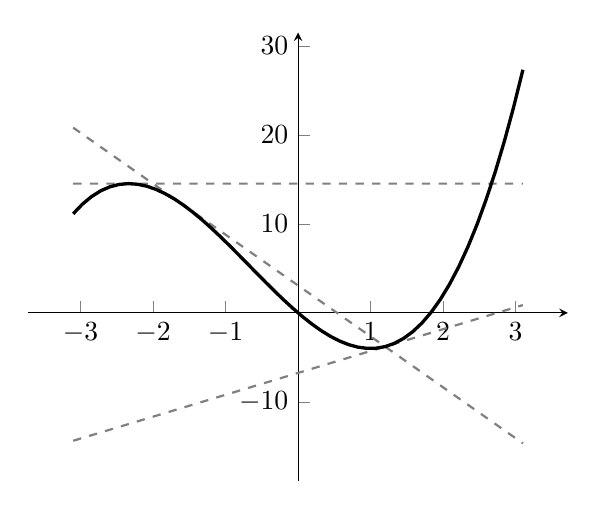
\begin{tikzpicture}[
                  declare function = {
                    f(\x) = (\x + 1)^3 - (\x - 1)^2 - 12 * \x;
                    dfx(\x) = 3*(\x + 1)^2 - 2*(\x - 1) - 12;
                    t1x(\x) = dfx(-1.6) * (\x + 1.6) + f(-1.6);
                    t2x(\x) = dfx(-7/3) * (\x + 7/3) + f(-7/3);
                    t3x(\x) = dfx(1.23) * (\x - 1.23) + f(1.23);
                  }
                ]
                \begin{axis}[
                  axis lines=center,
                  enlargelimits,
                  tick align=inside,
                  domain=-3.1:3.1,
                  samples=50,
                ]
                  \addplot +[mark=none, line width=0.8, color=gray, dashed] {t1x(x)};
                  \addplot +[mark=none, line width=0.8, color=gray, dashed] {t2x(x)};
                  \addplot +[mark=none, line width=0.8, color=gray, dashed] {t3x(x)};
                  \addplot +[mark=none, line width=1.2, color=black] {f(x)};
                \end{axis}
              \end{tikzpicture}
              \caption{%
                Graph of the $f(x) = (x+1)^3 - (x-1)^2 - 12 \cdot x$ function
                from example \ref{parsinglevarexample}, with its tangent lines
                at $x=-1.6$, at $x=-\frac{7}{3}$, and at $x=1.23$. The slopes
                of the tangent lines are given by
                $f'(-1.6)$, $f'(-\frac{7}{3})$, and $f'(1.23)$ respectively.
                The function has a local maximum at $x=-\frac{7}{3}$, so the
                tangent line there is horizontal, ie. its slope is $0$, ie.
                $f'(-\frac{7}{3}) = 0$.
              } \label{figsinglevarfunc}
            \end{figure}

            This function is differentiable on the entire $\mathbb{R}$ (proof
            left for the reader). A step by step calculation of its derivative:

            \begin{align*}
              f'(x) & = \left( (x+1)^3 - (x-1)^2 - 12 \cdot x \right)' \\
                    & = \left( (x+1)^3 - (x-1)^2 \right)' - (12 \cdot x)' \\
                    & = \left( (x+1)^3 \right)'
                        -
                        \left( (x-1)^2 \right)'
                        - (12 \cdot x)' \\
                    & = \left( (x+1)^3 \right)'
                        -
                        \left( (x-1)^2 \right)'
                        - 12 \cdot (x)' \\
                    & = \left( 3 \cdot (x+1)^2 \cdot (x+1)' \right)
                        -
                        \left( 2 \cdot (x-1) \cdot (x-1)' \right)
                        - 12 \cdot 1 \\
                    & = \left(
                          3 \cdot (x+1)^2 \cdot \left( (x)' + (1)' \right)
                        \right)
                        -
                        \left(
                          2 \cdot (x-1) \cdot \left( (x)' - (1)' \right)
                        \right)
                        - 12 \\
                    & = \left(
                          3 \cdot (x+1)^2 \cdot \left( 1 + 0 \right)
                        \right)
                        -
                        \left(
                          2 \cdot (x-1) \cdot \left( 1 - 0 \right)
                        \right)
                        - 12 \\
                    & = \left( 3 \cdot (x+1)^2 \cdot 1 \right)
                        -
                        \left( 2 \cdot (x-1) \cdot 1 \right)
                        - 12 \\
                    & = 3 \cdot (x+1)^2 - 2 \cdot (x-1) - 12
            \end{align*}

        \subsubsection{%
          Partial derivatives of multivariable, real-valued functions
          ($\frac{\partial}{\partial x_i} f(\mathbf{a})$)
        }

          For $n \in \mathbb{N}^+$, let $f : \mathbb{R}^n \rightarrow \mathbb{R}$
          be a function which maps vectors from $R^n$ to real numbers.

          For $n > i \in \mathbb{N}^+$, the partial derivative of $f$ in the
          direction $x_i$ at $\mathbf{a}$ is the following limit:

          \begin{equation} \label{eqpartdev}
            \frac{\partial}{\partial x_i} f(\mathbf{a})
              = \lim_{h \to 0}
                  \frac{
                    f(a_1, a_2, \ldots, a_i + h, \ldots, a_n)
                    - f(a_1, a_2, \ldots, a_i, \ldots, a_n)
                  }{
                    h
                  }
          \end{equation}

          Note: $\frac{\partial}{\partial x_i} f(\mathbf{a})$ can also be
          written as $\frac{\partial f}{\partial x_i} (\mathbf{a})$, and
          $\frac{\partial f}{\partial x_i} : \mathbb{R}^n \rightarrow \mathbb{R}$
          can be thought of as a function in its own right.

          The practical use of partial derivatives is that
          $\frac{\partial}{\partial x_i} f(\mathbf{a})$ tells the slope
          of the tangent line to the graph of $f$ at $\mathbf{a}$ along the
          axis that corresponds to the $x_i$ variable, similarly to the single
          variable case. (Figure \ref{figmultivarfunc1} in
          \ref{parmultivarexample} shows what this means for the $n=2$ case.)

          Since all the numbers in the expression in equation \ref{eqpartdev}
          are constants except for $a_i$, the expression can be treated just
          like a single variable function, and so the partial derivatives can be
          calculated the exact same way, with the exact same rules. In other
          words, if we define the $g : \mathbb{R} \rightarrow \mathbb{R}$
          single variable function for a given $\mathbf{a} \in \mathbb{R}^n$ and
          $n > i \in \mathbb{N}^+$ as
          $g(x) = f(a_1, a_2, \ldots, x, \ldots, a_n)$ with $x$ being the $i$-th
          parameter of $f$, then
          $\frac{\partial}{\partial x_i} f(\mathbf{a}) = g'(a_i)$.

          \paragraph{Gradient vector ($\nabla f(\mathbf{a})$)}

            For a given $\mathbf{a} \in \mathbb{R}^n$ vector, if all the
            partial derivatives $\frac{\partial}{\partial x_i}$ (for
            $n \geq i \in \mathbb{N}^+$) of $f$ are defined at $\mathbf{a}$,
            then the gradient of $f$ at $\mathbf{a}$ is the following vector
            ($\nabla f(\mathbf{a}) \in \mathbb{R}^n$):

            \begin{align*}
              \nabla f(\mathbf{a})
                = \left[
                    \frac{\partial}{\partial x_i} f(\mathbf{a})
                  \right]_{i=1}^n
                = \begin{bmatrix}
                    \vspace{1.5ex}
                    \frac{\partial}{\partial x_1} f(\mathbf{a}) \\
                    \frac{\partial}{\partial x_2} f(\mathbf{a}) \\
                    \vdots \\
                    \frac{\partial}{\partial x_n} f(\mathbf{a})
                  \end{bmatrix}
            \end{align*}

          \paragraph{Example}\label{parmultivarexample}

            Consider the following function:

            \begin{align*}
              f : & \mathbb{R}^2 \rightarrow \mathbb{R} \\
              f(x_1, x_2)
                = & \frac{1}{50}
                    \cdot
                    \left( (x_1 - 1)^3 - 5 \cdot x_2^{\enspace 2} \right) + 3
            \end{align*}

            Its graph is a 3-dimensional surface, as shown on figure
            \ref{figmultivarfunc1}, because this function can be thought of as
            if it assigned a height value for each point of a 2-dimensional
            plane.

            For example, the height of the surface above the
            $\mathbf{a} = \begin{bmatrix}3 \\ 1\end{bmatrix} \in \mathbb{R}^2$
            point on the plane is
            $
              f(3, 1)
                = \frac{1}{50} \cdot \left( (3-1)^3 - 5 \cdot 1^2 \right) + 3
                = 3.06
            $.

            \begin{figure}[!htb]
              \centering
              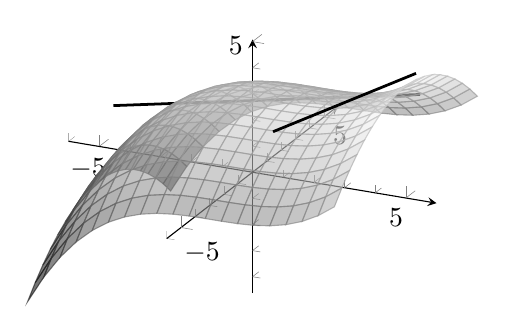
\begin{tikzpicture}[
                  declare function = {
                    f(\x,\y) = ((\x-1)^3 - 5*(\y^2)) / 50 + 3;
                    dfx1(\x) = (3/50) * (\x-1)^2;
                    dfx2(\x) = (-1/5) * \x;
                    tx1(\x) = dfx1(3) * (\x - 3) + f(3, 1);
                    tx2(\x) = dfx2(1) * (\x - 1) + f(3, 1);
                  }
                ]
                \begin{axis}[
                  axis lines=center,
                  enlargelimits,
                  tick align=inside,
                  domain=-5:5,
                  samples=20,
                  minor tick num=4,
                  colormap/blackwhite
                ]
                  \addplot3 +[mark=none, color=black, line width=1] (x, 1, {tx1(x)});
                  \addplot3 [surf, z buffer=sort, opacity=0.6] {f(x,y)};
                  \addplot3 +[mark=none, color=black, line width=1] (3, y, {tx2(y)});
                \end{axis}
              \end{tikzpicture}
              \caption{%
                Graph of the $f : \mathbb{R}^2 \rightarrow \mathbb{R}$,
                $
                  f(x_1, x_2)
                    = \frac{1}{50}
                      \cdot
                      \left( (x_1 - 1)^3 - 5 \cdot x_2^{\enspace 2} \right) + 3
                $
                function, and its tangent lines at
                $\mathbf{a} = \begin{bmatrix} 3 \\ 1 \end{bmatrix}$,
                parallel with the $x_1$ and $x_2$ axis, as given by
                $\nabla f(\mathbf{a})$.
              } \label{figmultivarfunc1}
            \end{figure}

            The partial derivatives exist for both of its variables. (Proof
            left for the reader.)

            If we slice this surface along the $x_2 = 1$ line which lies on the
            plane (this line is parallel to the $x_1$ axis), then we get the
            first graph that is shown on figure \ref{figmultivarfunc2}, and
            $\frac{\partial}{\partial x_1} f(3, 1)$ will tell the slope of the
            tangent line to this graph at the $x_1 = 3$ point. In other words,
            if we define the $g : \mathbb{R} \rightarrow \mathbb{R}$ function as
            $
              g(x_1) = f(x_1, a_2)
                = \frac{1}{50} \cdot \left( (x_1 - 1)^3 - 5 \cdot 1^2 \right) + 3
            $, then $g$ can be differentiated as a single variable function, and
            $\frac{\partial}{\partial x_1} f(\mathbf{a}) = g'(a_1)$.

            Similarly, slicing this function along the $x_1 = 3$ line (which is
            parallel to the $x_2$ axis) gives the second graph that is shown on
            figure \ref{figmultivarfunc2}, and
            $\frac{\partial}{\partial x_2} f(3, 1)$ will tell the slope of the
            tangent line to this graph at the $x_2 = 1$ point. In other words,
            if we define the $h : \mathbb{R} \rightarrow \mathbb{R}$ function as
            $
              h(x_2) = f(a_1, x_2)
                = \frac{1}{50}
                  \cdot
                  \left( (3 - 1)^3 - 5 \cdot x_2^{\enspace 2} \right)
                  +
                  3
            $, then $h$ can be differentiated as a single variable function as
            well, and $\frac{\partial}{\partial x_2} f(\mathbf{a}) = h'(a_2)$.

            \begin{figure}[!htb]
              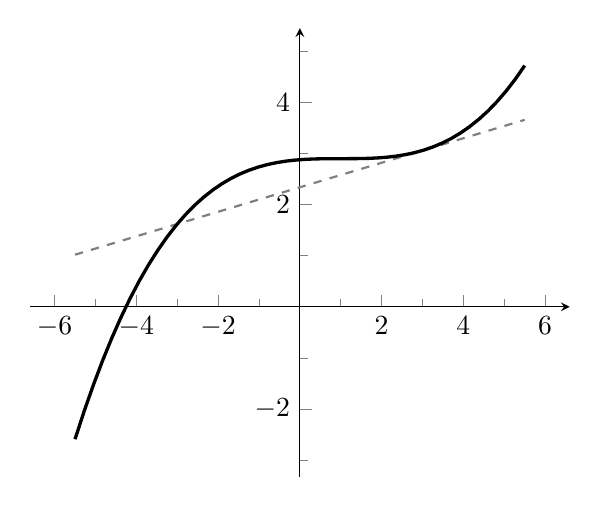
\begin{tikzpicture}[
                  declare function = {
                    f(\x) = ((\x-1)^3 - 5*1^2) / 50 + 3;
                    dfx1(\x) = 3/50 * (\x - 1)^2;
                    tx1(\x) = dfx1(3) * (\x - 3) + f(3);
                  }
                ]
                \begin{axis}[
                  axis lines=center,
                  enlargelimits,
                  tick align=inside,
                  domain=-5.5:5.5,
                  samples=50,
                  minor tick num=1,
                ]
                  \addplot +[mark=none, line width=0.8, color=gray, dashed] {tx1(x)};
                  \addplot +[mark=none, line width=1.2, color=black] {f(x)};
                \end{axis}
              \end{tikzpicture}
              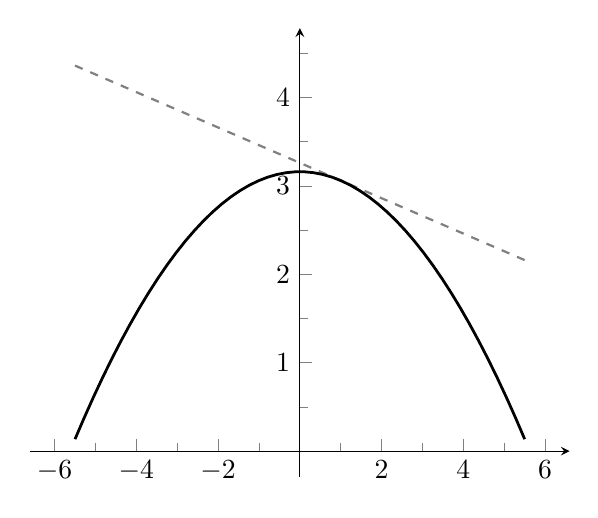
\begin{tikzpicture}[
                  declare function = {
                    f(\x) = ((3-1)^3 - 5*(\x^2)) / 50 + 3;
                    dfx2(\x) = (-1/5) * \x;
                    tx2(\x) = dfx2(1) * (\x - 1) + f(1);
                  }
                ]
                \begin{axis}[
                  axis lines=center,
                  enlargelimits,
                  tick align=inside,
                  domain=-5.5:5.5,
                  samples=50,
                  minor tick num=1,
                ]
                  \addplot +[mark=none, line width=0.8, color=gray, dashed] {tx2(x)};
                  \addplot +[mark=none, line width=1, color=black] {f(x)};
                \end{axis}
              \end{tikzpicture}
              \caption{%
                Graphs of the
                $
                  g(x_1) = f(x_1, a_2)
                    = \frac{1}{50}
                      \cdot
                      \left( (x_1 - 1)^3 - 5 \cdot 1^2 \right)
                      +
                      3
                $
                and the
                $
                  h(x_2) = f(a_1, x_2)
                    = \frac{1}{50}
                      \cdot
                      \left( (3 - 1)^3 - 5 \cdot x_2^{\enspace 2} \right)
                      +
                      3
                $
                slices of the $f$ function, and the tangent lines of these
                slices at $x_1 = 3$ and at $x_2 = 1$, as given by
                $\frac{\partial}{\partial x_1} f(3, 1)$ and
                $\frac{\partial}{\partial x_2} f(3, 1)$ respectively.
              } \label{figmultivarfunc2}
            \end{figure}

            Below is the calculation of the partial derivatives for the
            $\mathbf{a} = \begin{bmatrix}3 \\ 1\end{bmatrix}$ point, step by
            step. We are going to use the single value differentiation rules,
            and the fact that if $\alpha \in \mathbb{R}$ is a constant, then
            $(\alpha - 1)^3$ and $5 \cdot \alpha^2$ are also constants,
            therefore their derivatives are $0$.

            \begin{align*}
              \frac{\partial}{\partial x_1} f(x_1, a_2)
                & = \left(
                      \frac{1}{50}
                      \cdot
                      \left( (x_1 - 1)^3 - 5 \cdot a_2^{\enspace 2} \right)
                      +
                      3
                    \right)' \\
                & = \left(
                      \frac{1}{50}
                      \cdot
                      \left( (x_1 - 1)^3 - 5 \cdot a_2^{\enspace 2} \right)
                    \right)'
                    +
                    (3)' \\
                & = \left(
                      \frac{1}{50}
                      \cdot
                      \left( (x_1 - 1)^3 - 5 \cdot a_2^{\enspace 2} \right)
                    \right)'
                    +
                    0 \\
                & = \left(
                      \frac{1}{50}
                      \cdot
                      \left( (x_1 - 1)^3 - 5 \cdot a_2^{\enspace 2} \right)
                    \right)' \\
                & = \frac{1}{50}
                    \cdot
                    \left( (x_1 - 1)^3 - 5 \cdot a_2^{\enspace 2} \right)' \\
                & = \frac{1}{50}
                    \cdot
                    \left(
                      \left(
                        (x_1 - 1)^3 \right)' - \left(5 \cdot a_2^{\enspace 2}
                      \right)'
                    \right) \\
                & = \frac{1}{50}
                    \cdot
                    \left( \left( (x_1 - 1)^3 \right)' - 0 \right) \\
                & = \frac{1}{50}
                    \cdot
                    \left( (x_1 - 1)^3 \right)' \\
                & = \frac{1}{50}
                    \cdot
                    \left(
                      3 \cdot (x_1 - 1)^2 \cdot \left( x_1 - 1 \right)'
                    \right) \\
                & = \frac{1}{50}
                    \cdot
                    \left(
                      3 \cdot (x_1 - 1)^2 \cdot \left( (x_1)' - (1)' \right)
                    \right) \\
                & = \frac{1}{50}
                    \cdot
                    \left( 3 \cdot (x_1 - 1)^2 \cdot (1 - 0) \right) \\
                & = \frac{1}{50}
                    \cdot
                    \left( 3 \cdot (x_1 - 1)^2 \cdot 1 \right) \\
                & = \frac{3}{50} \cdot (x_1 - 1)^2 \\
            \end{align*}

            Now $\frac{\partial}{\partial x_2} f(a_1, x_2)$ with somewhat bigger
            steps:

            \begin{align*}
              \frac{\partial}{\partial x_2} f(a_1, x_2)
                & = \left(
                      \frac{1}{50}
                      \cdot
                      \left( (a_1 - 1)^3 - 5 \cdot x_2^{\enspace 2} \right) + 3
                    \right)' \\
                & = \left(
                      \frac{1}{50}
                      \cdot
                      \left( (a_1 - 1)^3 - 5 \cdot x_2^{\enspace 2} \right)
                    \right)'
                    +
                    (3)' \\
                & = \frac{1}{50}
                    \cdot
                    \left( (a_1 - 1)^3 - 5 \cdot x_2^{\enspace 2} \right)'
                    +
                    0 \\
                & = \frac{1}{50}
                    \cdot
                    \left(
                      \left(
                        (a_1 - 1)^3 \right)'
                        - \left(5 \cdot x_2^{\enspace 2} \right)'
                    \right) \\
                & = \frac{1}{50}
                    \cdot
                    \left(
                      0 - 5 \cdot \left( x_2^{\enspace 2} \right)'
                    \right) \\
                & = \frac{1}{50}
                    \cdot
                    (-5)
                    \cdot
                    \left( x_2^{\enspace 2} \right)' \\
                & = - \frac{1}{10}
                    \cdot
                    \left( 2 \cdot x_2 \cdot \left( x_2 \right)' \right) \\
                & = - \frac{1}{10}
                    \cdot
                    \left( 2 \cdot x_2 \cdot 1 \right) \\
                & = - \frac{1}{5} \cdot x_2
            \end{align*}

            Therefore the gradient vector at the
            $\mathbf{a} = \begin{bmatrix}3 \\ 1\end{bmatrix} \in \mathbb{R}^2$
            point is:

            \begin{align*}
              \nabla f(\mathbf{a})
                = \begin{bmatrix}
                    \vspace{1.5ex}
                    \frac{\partial}{\partial x_1} f(3, 1) \\
                    \frac{\partial}{\partial x_2} f(3, 1)
                  \end{bmatrix}
                = \begin{bmatrix}
                    \vspace{1.5ex}
                    \frac{3}{50} \cdot (3 - 1)^2 \\
                    - \frac{1}{5} \cdot 1
                  \end{bmatrix}
                = \begin{bmatrix}
                    \vspace{1.5ex}
                    \frac{6}{25} \\
                    - \frac{1}{5}
                  \end{bmatrix}
            \end{align*}

            Note: the math works the same way for more than 2 dimensions
            ($n > 2$), it's just harder to visualize.

\end{document}
